

\chapter{Konstruktiver Entwicklungsprozess des Prüfstandes}\label{cha:3}

Für die vorliegende Arbeit soll soweit möglich der in der Fachliteratur wie bspw. der Konstruktionslehre nach Pahl und Beitz~\cite{Pahl_Beitz_Konstruktionslehre} oder der VDI~2222~\cite{VDI_2222-1} schematisierte kontruktive Entwicklungsprozess Anwendnung finden. Die Darstellung des Entwicklungsprozesses erfolgt weiterhin in Anlehung an~\cite{Projektarbeit}.
\par
\vspace{\linespace}
Der Synthese einer konstruktiven Lösung geht die Analyse der Aufgabenstellung hinsichtlich der gestellten Anforderungen voraus, deren Ergebnis eine Anforderungsliste ist. Dadurch wird sichergestellt, dass der Entwicklungsprozess alle Forderungen erfüllt. Das in der anschließenden Konzeptphase entstandene Konzept wird dann im Verlauf der Entwurfsphase in eine quantitative Gestaltung überführt. Im Rahmen der letzten Entwicklungsphase, der Ausarbeitung, werden die verbliebenen Feinheiten zur Erfüllung der Anforderungen eingearbeitet. Die fertig ausgearbeitete Lösung schließt den Entwicklungsprozess ab.
\par
\vspace{\linespace}
Eine klare Trennung der beschriebenen Phasen kann in der Praxis jedoch selten erfolgen. Hinzu kommt das Durchlaufen mehrerer Iterationsschleifen, bei denen die gestellten Anforderungen stets durch neu erhaltene Informationen und die vorangeschrittene Entwicklung weiter präzisiert und soweit wie möglich mit konkreten Werten belegt werden. Im Folgenden soll das Ergebnis des konstruktiven Entwicklungsprozesses kurz dargestellt und erläutert werden.   


\section{Präzisierung der Aufgabenstellung}\label{cha:3_Praezisierung_Aufgabenstellung}




Im Verlauf der Aufgabenanalyse erfolgt die Erstellung einer Anforderungsliste, welche die Forderungen an die Konstruktion möglichst umfangreich zusammenstellt. Die Anforderungen setzen sich hauptsächlich aus den Rahmenbedingungen und Wünschen hinsichtlich verschiedener Hauptmerkmale und zur Funktionserfüllung notwendigen Forderungen zusammen. In Anlehnung an die Kategorisierung, wie sie in der Literatur beschrieben wird, wurde die Unterteilung in \acp{F} und \acp{W} vorgenommen. Dadurch konnten Anforderungen identifiziert werden, die durch alle Konzepte unbedingt zu erfüllen sind und solche, die nach Möglichkeit Berücksichtigung finden sollten. Der Erfüllungsgrad aller Anforderungen bildete die Bewertungsgrundlage der Konzeptideen.
\par
\vspace{\linespace}
Die Präzisierung der Detailanforderungen erfolgte teilweise und insofern möglich in Iterationsschleifen während der Konzept- und Entwurfsphase, wobei hier nur das Ergebnis dargestellt werden soll. Die Anforderungsliste im \Anhang\ref{A:Anforderungsliste} enthält die  soweit möglich konkretisierten Anforderungen sowie zusätzlich und falls notwendig eine Bemerkung zur Hauptquelle für die Präzisierung.
\par
\vspace{\linespace}
Der Fokus der Entwicklung soll vor allem auf einer hohen Wiederholbarkeit der Messungen liegen, da eine Abschätzung der Reproduzierbarkeit aufgrund von geometrischen Abweichungen und unterschiedlichen Antennencharakteristika im Voraus so gut wie nicht möglich ist (vgl. \Abschnitt\ref{cha:2_Methoden_der_Schirmdaempfungsmessung}).









\section{Konstruktion kommerzieller Absorberkammern}\label{cha:3_Konstruktion_kommerzieller_Absorberkammern}



Geschirmte Räume bzw. Absorberkammern werden im kommerziellen Sektor von vielen Herstellern benötigt, da der Test auf elektromagnetische Verträglichkeit von Betriebsmitteln u.a. Teil der CE"=Kennzeichnung~\cite{Richtlinie_2014/30/EU} ist. Gängig sind dabei große Räume, die oft von unabhängigen Testzentren betrieben werden und eine große Bandbreite von Geräten und Betriebsmitteln testen können. Die Testräume bestehen dabei im Allgemeinen aus einzelnen Modulen oder die Schirmung wird direkt in die Wand eines Gebäudes integriert~\cite{EM_Schirmung}. Im Folgenden wird die Modulbauweise näher betrachtet.
\par
\vspace{\linespace}
Grundsätzlich sind zwei Bauweisen von Schirmkabinen üblich: Gekantete Stahlbleche, die miteinander verschraubt werden, und Verbundplatten aus metallischen Deckblechen mit einem Kern aus Pressspan, die durch Profile miteinander verbunden werden~\cite{EM_Schirmung, Design_of_shielded_enclosures}. In \Abb\ref{fig:3_Allgemeiner_Aufbau_Schirmkabinen} sind beide Varianten schematisch dargestellt. Alle im Rahmen der Recherche betrachteten Anbieter geschirmter Räume bzw. Messkabinen verwendeten eine dieser Varianten ohne nennenswerte Abwandlung.

\begin{figure}[H]
    \centering
    \begin{subfigure}[b]{0.4\textwidth}
        \includegraphics[page = 2, height=0.14\textheight,trim = 8.5cm 5.5cm 8.5cm 4.5cm, clip]{Abbildungen/Kapitel3/Schirmkabinen.pdf}
        \caption{Stahlblechplatten\label{subfig:3_Aufbau_Stahlblechkabine}}
    \end{subfigure}
    \hspace{1cm}
    \begin{subfigure}[b]{0.5\textwidth}
        \includegraphics[page = 3, height=0.135\textheight, trim = 11.5cm 6.5cm 7cm 6cm, clip]{Abbildungen/Kapitel3/Schirmkabinen.pdf}
        \caption{Sandwichmodule\label{subfig:3_Aufbau_Sandwichkabine}}
    \end{subfigure}
    %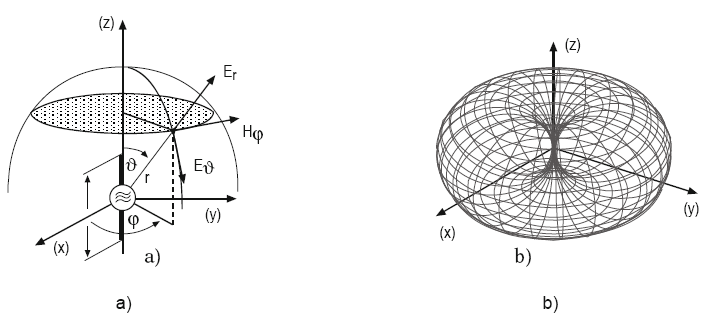
\includegraphics[width=.8\textwidth]{Abbildungen/Kapitel2/Feldverlauf.png}
    \caption[Schematischer Aufbau von Schirmkabinen]{Schematischer Aufbau von Schirmkabinen nach~\cite{EMC-Technik_Stahlblechplatten, EMC-Technik_Sandwichmodul, EM_Schirmung, Design_of_shielded_enclosures}}
    \label{fig:3_Allgemeiner_Aufbau_Schirmkabinen}
\end{figure}

Der Vorteil verschraubter Stahlblechwannen ist offensichtlich die hohe Haltbarkeit der Verschraubung. Allerdings ist die erreichbare Schirmdämpfung sehr sensitiv bezüglich der korrekten Lage der Hochfrequenz"=Dichtungen (HF-Dichtungen) zwischen den Blechplatten. Weiterhin neigen diese Module zum Vibrieren und je nach Größe ist zusätzlich eine Außenkonstruktion für die Selbsttragfähigkeit des Schirmkabine notwendig~\cite{EM_Schirmung}.
\par
\vspace{\linespace}
Ein System aus Verbund- oder Sandwich-Paneelen ist selbsttragend und benötigt aufgrund der überlappenden Profile zwischen den einzelnen Modulen keine HF-Dichtungen. Als Nachteil ist hier vor allem zu nennen, dass die unsachgemäße Verschraubung bei Verwendung selbstschneidender Schrauben zu Lecks führen kann, weil die Anpressung der Profile an die Modulwände stellenweise nicht mehr gegeben ist~\cite{EM_Schirmung}. 
\par
\vspace{\linespace}
Bei vergleichbarer Größe und Ausstattung sind Kabinen aus Sandwich-Modulen im Allgemeinen günstiger als solche aus Stahlblechplatten~\cite{EMC-Technik_Sandwichmodul, EMC-Technik_Stahlblechplatten}. Dies und die Sensitivität der Stahlblechkonstruktion (vgl. \Abb\ref{subfig:3_Aufbau_Stahlblechkabine}) gegenüber der korrekten Lage der HF-Dichtungen waren unter anderem ausschlaggebend für die Wahl der Sandwichbauweise für den Aufbau der Modulwände. Im folgenden \Abschnitt\ref{cha:3_Konzepterstellung} wird auf die Konzeptauswahl näher eingegangen.  %Deshalb und aufgrund der Sensitivität gegenüber der korrekten Lage der HF-Dichtungen soll die Konstruktion im Rahmen dieser Arbeit in Anlehnung an die Sandwich-Modulbauweise erfolgen. 








\section{Konzepterstellung}\label{cha:3_Konzepterstellung}




\subsection{Funktionsstruktur und Konzeptbewertung}

Ein Konzept stellt in erster Linie einen prinzipiellen Aufbau dar und dient der Überprüfung, inwieweit die gestellten Anforderungen erfüllt wurden. Da durch das Konzept die grundlegende Gestalt und die wichtigsten Merkmale festgelegt werden, ist die Konzeptphase einer der wichtigsten Abschnitte im Entwicklungsprozess. Das Gesamtkonzept lässt sich nach~\cite{Pahl_Beitz_Konstruktionslehre} folgendermaßen unterteilen:

\begin{description}
    \item[Gestaltungskonzept] Festlegung der grundlegenden Geometrie, Zuordnung der einzelnen Komponenten und Betrachtung von Stoff-, Energie- und Signalflüssen
    \item[Wirkkonzept] Beschreibung der physikalischen Effekte und deren Verknüpfung zur Erfüllung der gestellten Anforderungen sowie der Gestalt der Wirkflächen
    \item[Wirkfläche] Funktionale Flächen, an denen das Wirkkonzept umgesetzt wird
\end{description}

Unter Berücksichtigung der Forderungen, welche die Funktion unmittelbar beeinflussen, wurden zunächst die wesentlichen Aufgaben der Konstruktion identifiziert. Die Gesamtaufgabe ist bereits eindeutig festgelegt: Innerhalb einer von äußeren Störeinflüssen abgeschirmten Messkabine sollen Probekörper im Koppelpfad zweier Hornantennen positioniert werden, wobei durch die geometrischen Abmessungen und die Verkleidung reflektiver Flächen im Inneren der Messkammer sichergestellt werden soll, dass sich die Proben im ungestörten Fernfeld (vgl. \Kapitel\ref{cha:2}) der Antennen befinden. Festzulegen bleibt im Weiteren der genaue Aufbau der Messkabine unter Berücksichtigung der zu erreichenden Schirmung, die Gestaltung von Öffnungen und Durchführungen, die Positionierung der Antennen und Probekörper und die Auswahl geeigneter Absorber, um Hohlraumresonanzen (vgl. \Abschnitt\ref{cha:2_subsub_Hohlraumresonanzen}), Reflektionen und indirekte Kopplung (vgl. \Abschnitt\ref{cha:2_sub_Reflektion}) zu vermeiden. Mithilfe der in \Abb\ref{fig:3_Funktionsstruktur} dargestellten Funktionsstruktur wurde die Gesamtaufgabe weiter abstrahiert und gegliedert. %Die Qualifikation des Teststandes anhand des Vergleiches der durchgeführten und mit früheren Messungen ist als Teil der Auswertung nicht in der Funktionsstruktur enthalten.

\begin{figure}[ht]
    \centering
    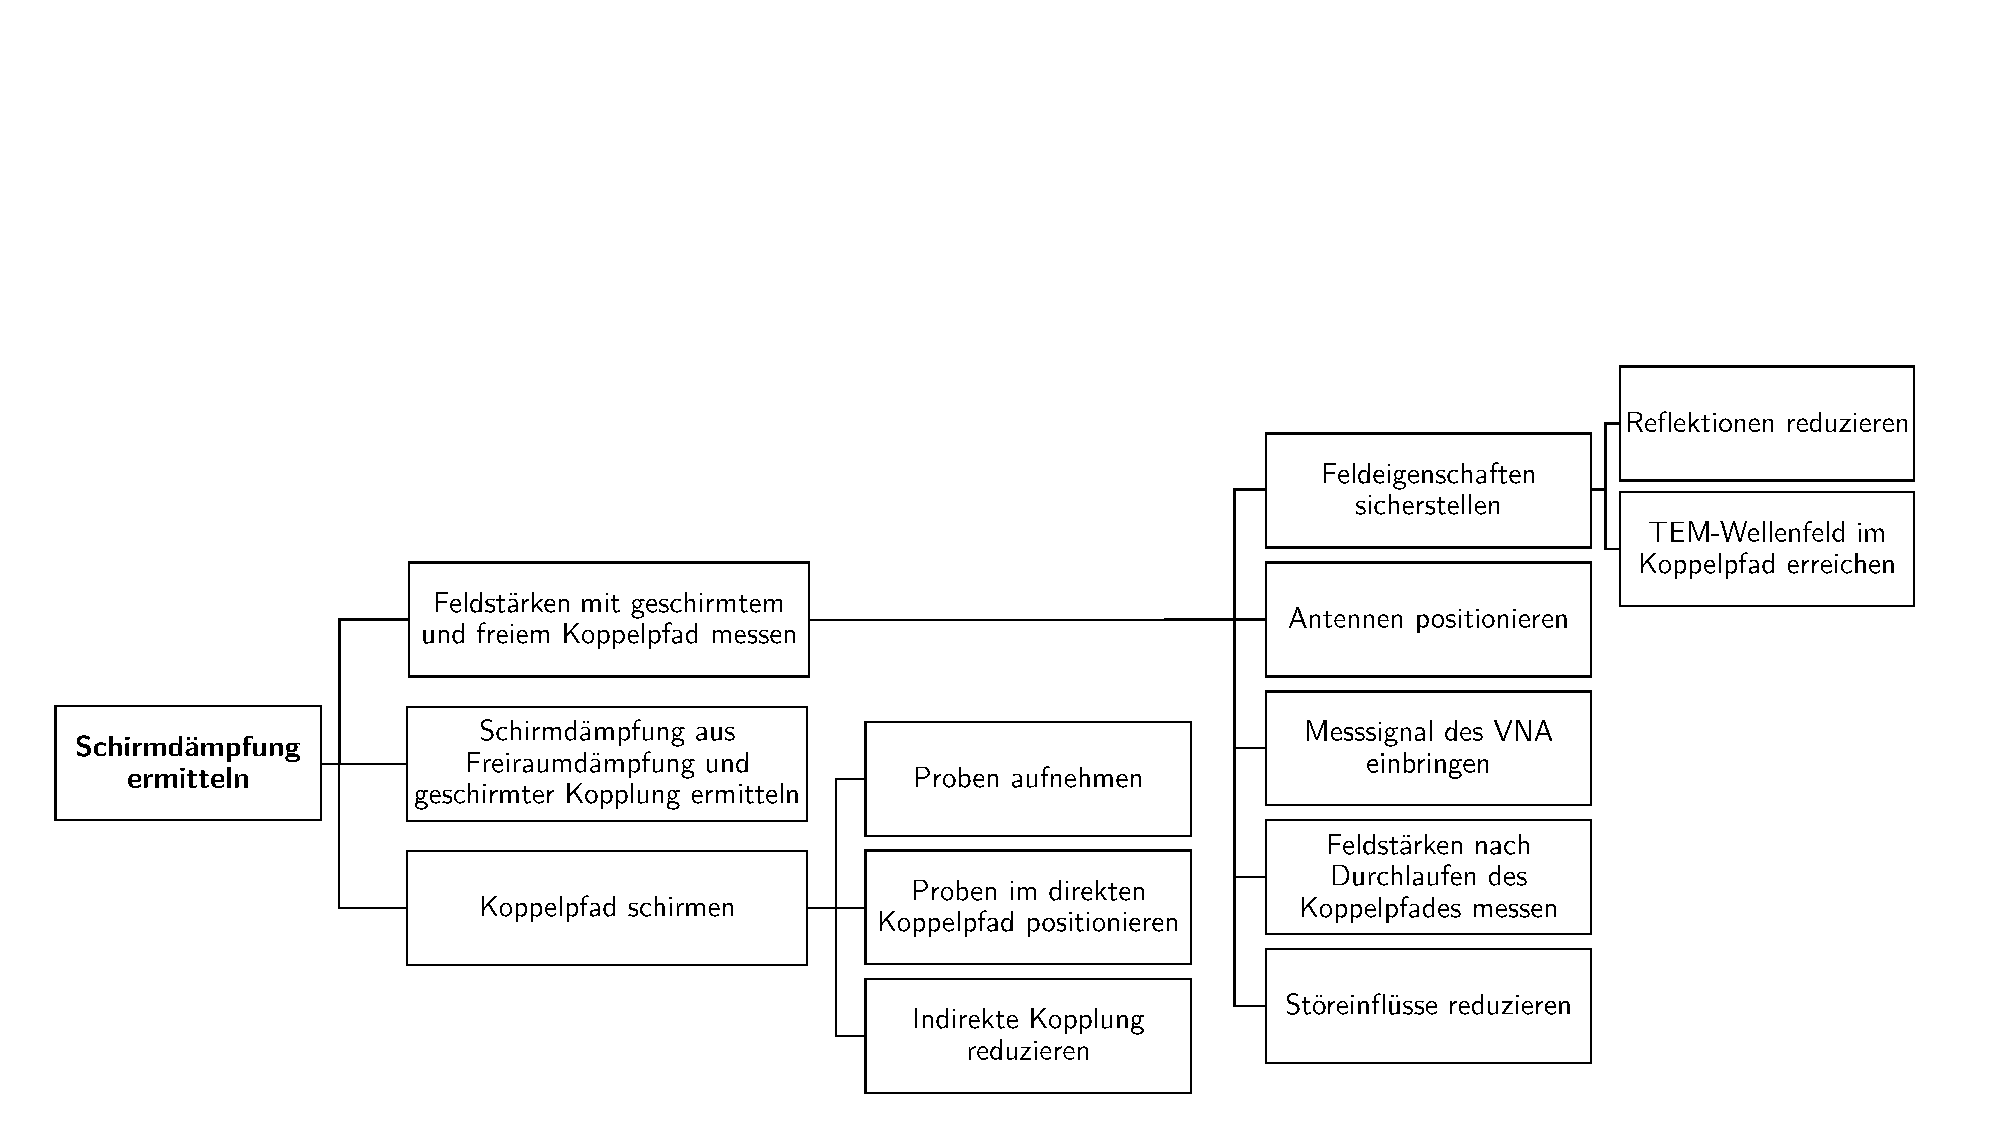
\includegraphics[page = 1, width=\textwidth, trim = 0.8cm 0.5cm 1.3cm 5.5cm, clip]{Abbildungen/Kapitel3/Funktionsstruktur.pdf}
    \caption{Funktionsstruktur der Messkabine}
    \label{fig:3_Funktionsstruktur}
\end{figure}


Auf dieser Grundlage lassen sich nun verschiedene Wirkkonzepte für die Teilstrukturen der Messkammer und deren Wirkflächen erstellen. Das Augenmerk des Designs lag dabei auf einer robusten und einfachen Geometrie der Wirkflächen bei gleichzeitiger Gewährleistung einer möglichst hohen Dichtheit gegenüber elektromagnetischer Strahlung. Letzteres kann nach der betrachteten Theorie in den \Abschnitten\ref{cha:2_sub_Daempfung_und_Absorption}, \ref{cha:2_sub_Reflektion} und \ref{cha:2_sub_Schirmung_ebener_Wellenfelder} durch die Herstellung eines leitfähigen Flächenkontaktes mit möglichst geringem Kontaktwiderstand zwischen allen Elementen der äußeren Schirmwand erreicht werden. Dies ist somit der physikalische Effekt, auf dem die Wirkkonzepte der Messkabine und der Durchführungen beruhen. 
\par
\vspace{\linespace}
Zur strukturierten und nachvollziehbaren Durchführung des Entscheidungsprozesses und der Auswahl der potenziell besten aus den vorgestellten Lösungsvarianten, kam ein Bewertungsschema zum Einsatz. Die Bewertungskriterien wurden nach dem Top-down-Vorgehen abgeleitet. Das beudeutet die Anforderungen des gesamten Versuchsstandes wurden für die einzelnen Teilsysteme detailliert~\cite{Pahl_Beitz_Konstruktionslehre}. Die gewählten Kriterien weisen die in~\cite{Pahl_Beitz_Konstruktionslehre} beschriebenen Voraussetzungen, wie unter anderem Freiheit von Dopplungen, Gegenläufigkeit und Widersprüchen sowie Gültigkeit für alle vorgestellten Varianten, auf.
\par
\vspace{\linespace}
Die Bewertung bestand aus der Anwendung eines gewichteten Punkteschemas, welches allen Kriterien Maßzahlen hinsichtlich ihrer Erfüllung durch die Konzepte zuordnete. Dies sorgte für ein vergleichsweise einfaches Bewertungsschema, welches gegenüber einer reinen Argumentenbilanz jedoch eine deutlich präzisere Entscheidung zulässt und die quantifizierbare Möglichkeit einer Wichtung bietet. Die Bewertung der einzelnen Konzepte erfolgte getrennt je Teilsystem des Aufbaus. Mithilfe des errechneten Gesamtwertes $G_V$ je Lösungsvariante aus den Maßzahlen $M$ und den Gewichtet $w$ konnte die Auswahl der besten Variante unmittelbar erfolgen~\cite{Pahl_Beitz_Konstruktionslehre}:

\begin{equation}
    G_{V_i} = \sum_{j=1}^{k} w_j \cdot M_{j,i}
    \label{eq:3_Gesamtwert_Variantenvergleich}
\end{equation}
\begin{equation}
    w_j \in \{\mathbb{Q} \;\vert\; 0 < w_j \leq 1\}; \qquad \sum_{j=1}^{k} w_j = 1; \qquad M_{j,i} \in \{1,\,2,\,3,\,4\}
    \label{eq:3_Wichtung_Bewertung}
\end{equation}
\begin{equation*}
    \text{\textit{k: Anzahl Kriterien; i: Variante; j: Kriterium}}
\end{equation*}

Eine höhere Maßzahl der Bewertung steht dabei stets für die jeweils bessere Variante innerhalb eines Kriteriums. Damit kann die beste Variante der jeweiligen Teilstruktur durch den höchsten Gesamtwert $G_V$ identifiziert werden. Die Wichtung erfolgte entsprechend der Kategorisierung und Wichtigkeit der jeweiligen Forderung.
\par
\vspace{\linespace}
Die Gestaltung der Probenhalterung als Teil der Messstrecke erfolgte ebenfalls im Rahmen der Konzeptphase. Die betrachteten Varianten wiesen jedoch nur geringe Unterschiede auf, sodass hier nur das gewählte Konzept als Teil des Entwurfes im \Abschnitt\ref{cha:3_Entwurf} beschrieben wird. Ähnliches gilt für die Auswahl geeigneter Absorberelemente zur Auskleidung des Innenraumes des Versuchsstandes und weitere Details, wie bspw. die Durchführungen der Antennenkabel, sodass diese und eine kurze Beschreibung der Entscheidungsgrundlage ebenfalls im \Abschnitt\ref{cha:3_Entwurf} vorgestellt werden.
%\par
%\vspace{\linespace}


\subsection{Schirmmodule des Versuchsstandes}\label{cha:3_sub_Schirmmodule_Versuchsstand}

Die Module bzw. Wände der Messkabine übernehmen die Schirmung äußerer Störeinflüsse und sind gleichzeitig Anschlussflächen zur Befestigung der Absorberelemente, Türen und Kabeldurchführungen. Bei den betrachteten Konzepten kann davon ausgegengen werden, dass ihre Schirmdämpfung im Idealfall deutlich größer als die der Durchführungen ist, sodass für die Bewertung entscheident war, wie robust diese Schirmdämpfung gegenüber Unebenheiten und Abweichungen ist. Beispielsweise bieten mehrere Wirkflächen, die in einer Art Labyrinth im Koppelpfad angeordnet sind auch dann noch eine ausreichende Schirmung, wenn eine der Wirkflächenpaarungen nicht korrekt aufeinander liegt und damit kein leitender über der gesamten Fläche entsteht. 
\par
\vspace{\linespace}
Die \Tabelle\ref{tab_3:Konzepte_Schirmmodule} zeigt die Wirkkonzepte, für welche die Bewertung durchgeführt wurde und aus denen das finale Konzept ausgewählt wurde. 


\begin{longtable}{l p{6.55cm} p{6.55cm}}
    \caption{Wirkkonzeptskizzen der Schirmmodule des Versuchsstandes}
    \vspace{\tablespace}
    \label{tab_3:Konzepte_Schirmmodule} \\
    \toprule 
    \textbf{Bauweise}& \multicolumn{2}{l}{\textbf{Varianten}}\\
    \midrule 
    \endfirsthead 
    \caption[]{Wirkkonzeptskizzen der Schirmmodule des Versuchsstandes \emph{(Fortsetzung)}}
    \vspace{\tablespace} \\
    \toprule 
    \textbf{Bauweise}& \multicolumn{2}{l}{\textbf{Varianten}}\\
    \midrule 
    \endhead 
    \bottomrule\nopagebreak 
    \multicolumn{3}{c}{\dots}
    \endfoot 
    \bottomrule 
    \endlastfoot

         \textbf{Stahlblech} & Variante 1 & Variante 2 \\ \nopagebreak
         & \noindent\begin{minipage}{6.5cm}
                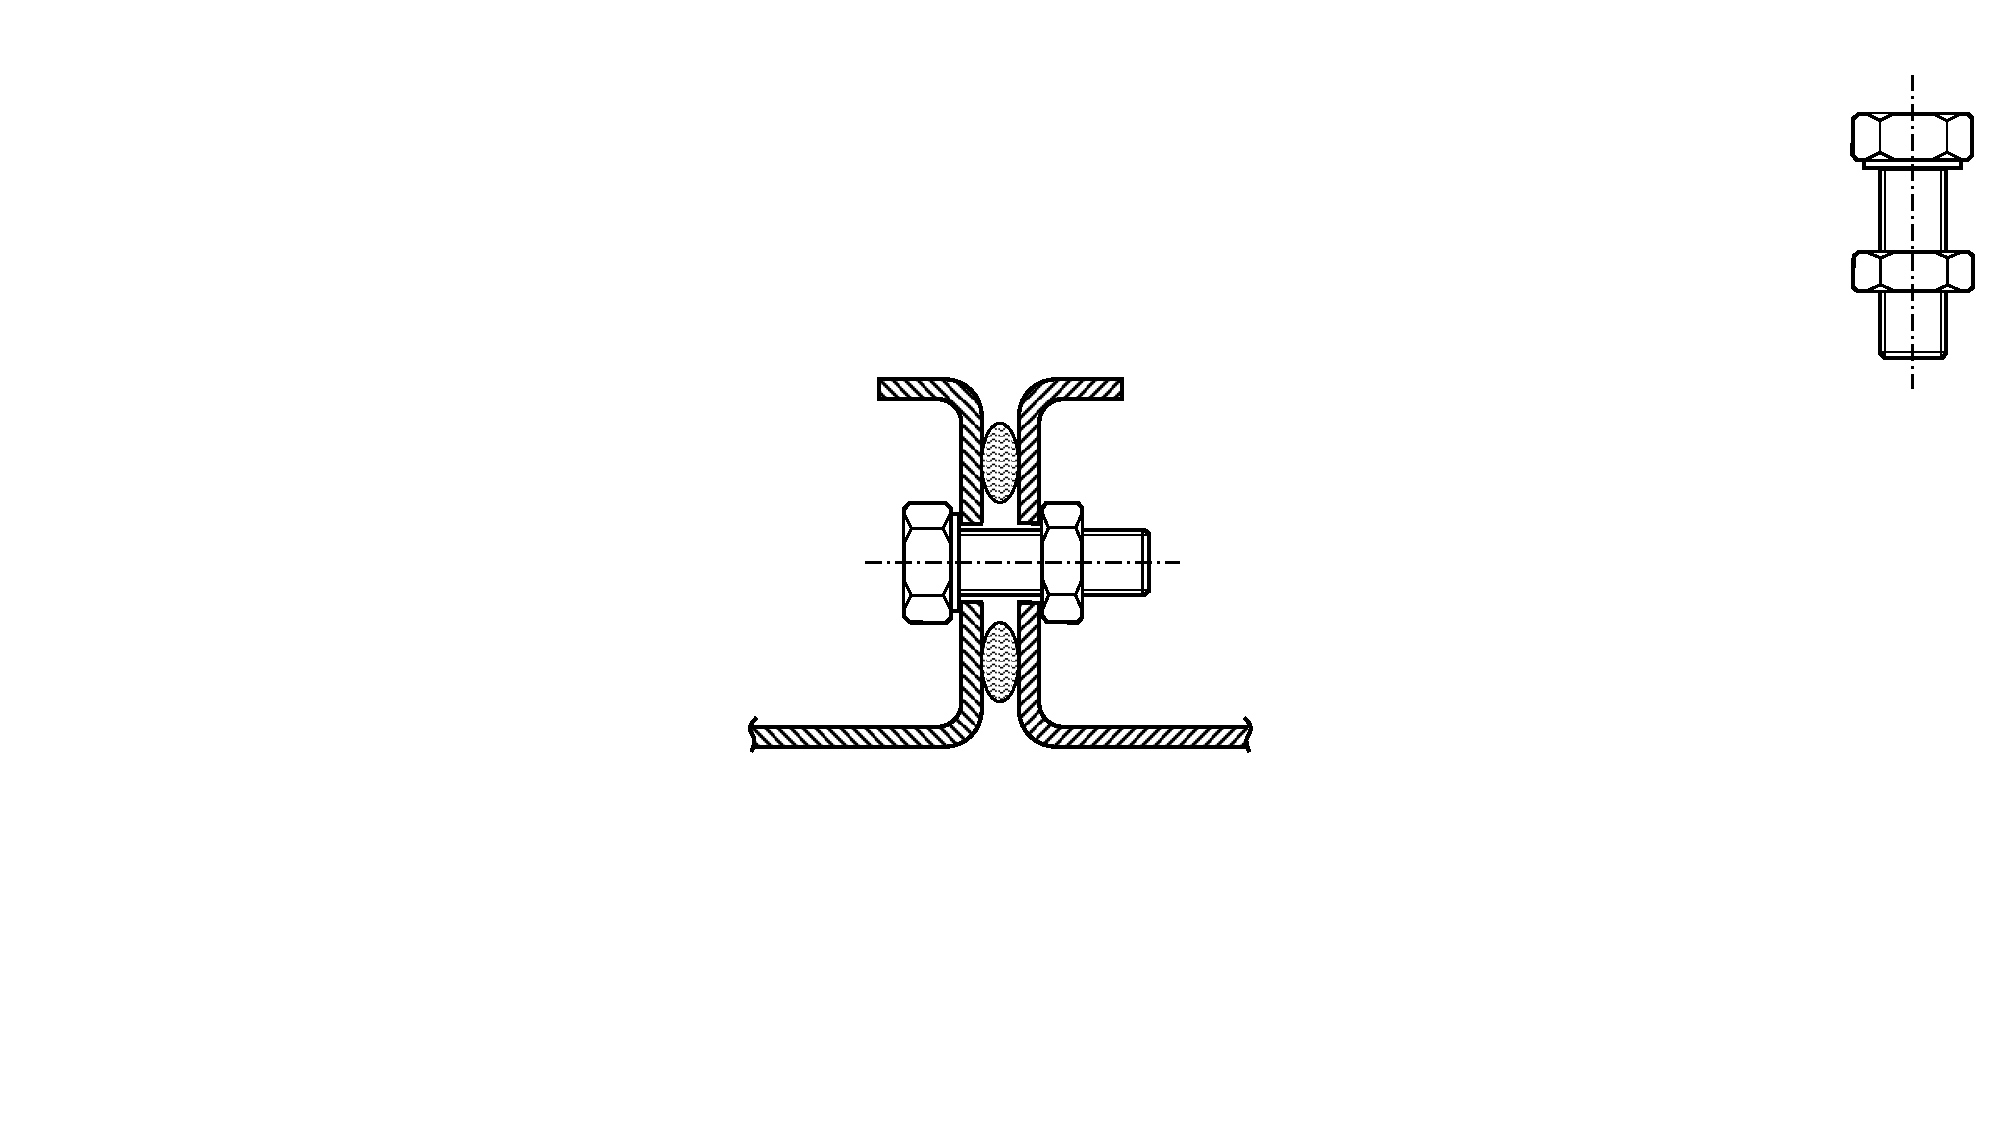
\includegraphics[page=1, width=0.95\textwidth, trim = 12cm 5.5cm 12cm 5.5cm, clip]{Abbildungen/Kapitel3/Konzepte.pdf}
        \end{minipage} &
        \noindent\begin{minipage}{6.5cm}
                \includegraphics[page=2, width=0.95\textwidth, trim = 12cm 5.5cm 12cm 5.5cm, clip]{Abbildungen/Kapitel3/Konzepte.pdf}
        \end{minipage} \\
         & Variante 3 & Variante 4 \\ \nopagebreak
         & \noindent\begin{minipage}{6.5cm}
                \includegraphics[page=3, width=0.95\textwidth, trim = 12cm 5.5cm 12cm 6.5cm, clip]{Abbildungen/Kapitel3/Konzepte.pdf}
        \end{minipage} &
        \noindent\begin{minipage}{6.5cm}
                \includegraphics[page=4, width=0.95\textwidth, trim = 12cm 6cm 12cm 5.5cm, clip]{Abbildungen/Kapitel3/Konzepte.pdf}
        \end{minipage} \\
    \midrule
         \textbf{Sandwich} & Variante 5 & Variante 6 \\ \nopagebreak 
         & \noindent\begin{minipage}{6.5cm}
                \includegraphics[page=5, width=0.95\textwidth, trim = 12.5cm 6cm 12cm 6cm, clip]{Abbildungen/Kapitel3/Konzepte.pdf}
        \end{minipage} &
        \noindent\begin{minipage}{6.5cm}
                \includegraphics[page=6, width=0.95\textwidth, trim = 14cm 7cm 10cm 7cm, clip]{Abbildungen/Kapitel3/Konzepte.pdf}
        \end{minipage} \\
         & Variante 7 & Variante 8  \\ \nopagebreak
         & \noindent\begin{minipage}{6.5cm}
                \includegraphics[page=7, width=0.95\textwidth, trim = 13cm 7cm 12cm 7cm, clip]{Abbildungen/Kapitel3/Konzepte.pdf}
        \end{minipage} &
        \noindent\begin{minipage}{6.5cm}
                \includegraphics[page=8, width=0.95\textwidth, trim = 8.5cm 3cm 12cm 5.5cm, clip]{Abbildungen/Kapitel3/Konzepte.pdf}
        \end{minipage} \\
\end{longtable}


\par
\vspace{\linespace}
Die Bewertung der verschiedenen Wirkkonzepte erfolgte anhand der nachstehenden \acp{K}: 

\begin{tabular}{l l}
    \centering
    \hspace*{1cm} \parbox[c][3cm]{7cm}{
        \begin{itemize}[]
            \item \textbf{K\textsubscript{1}} Materialkosten
            \item \textbf{K\textsubscript{2}} Fertigungsaufwand
            \item \textbf{K\textsubscript{3}} Robustheit gegenüber Lecks
        \end{itemize}
    }&
    \parbox[c]{7cm}{
        \begin{itemize}[]
            \item \textbf{K\textsubscript{4}} Montageaufwand
            \item \textbf{K\textsubscript{5}} Stabilität
            \item \textbf{K\textsubscript{6}} Materialverfügbarkeit
        \end{itemize}
    }
\end{tabular}

In der \Tabelle\ref{tab:3_Module_Messkabine} ist die Konzeptbewertung der Modulwände und die Auswertung nach den \Gleichungen\eqref{eq:3_Gesamtwert_Variantenvergleich} und \eqref{eq:3_Wichtung_Bewertung} dargestellt.


\begin{table}[ht]
    \centering
    \renewcommand{\arraystretch}{1.3}
    \caption{Konzeptbewertung der Schirmmodule des Versuchsstandes}
    \vspace{\tablespace}
    \label{tab:3_Module_Messkabine}
    \begin{tabularx}{\textwidth}{p{3cm} r C{1cm} C{1cm} C{1cm} C{1cm} C{1cm} C{1cm} C{1.5cm}}
        \toprule
        \multirow{2}{*}{\textbf{Variante i}} & \textbf{Kriterien K\textsubscript{j}} & \textbf{K\textsubscript{1}} & \textbf{K\textsubscript{2}} & \textbf{K\textsubscript{3}} & \textbf{K\textsubscript{4}} & \textbf{K\textsubscript{5}} & \textbf{K\textsubscript{6}} & \textbf{Summe} \\
         & Gewichte w\textsubscript{j} & 0,1 & 0,1 & 0,25 & 0,1 & 0,2 & 0,25 & \textbf{G\textsubscript{V}} \\
         \midrule
         \multicolumn{2}{l}{Variante 1} & 1 & 2 & 2 & 2 & 3 & 3 & 2,35 \\
         \multicolumn{2}{l}{Variante 2} & 2 & 3 & 2 & 3 & 2 & 3 & 2,45 \\
         \multicolumn{2}{l}{Variante 3} & 1 & 1 & 4 & 3 & 3 & 2 & 2,6 \\
         \multicolumn{2}{l}{Variante 4} & 2 & 2 & 4 & 4 & 2 & 2 & 2.7 \\
         \multicolumn{2}{l}{Variante 5} & 2 & 4 & 3 & 1 & 2 & 2 & 2,35 \\
         \multicolumn{2}{l}{Variante 6} & 4 & 4 & 4 & 2 & 3 & 1 & 2,85 \\
         \multicolumn{2}{l}{Variante 7} & 3 & 4 & 3 & 2 & 4 & 4 & 3,45 \\
         \multicolumn{2}{l}{Variante 8} & 3 & 2 & 1 & 3 & 1 & 4 & 2,25 \\
         \bottomrule
    \end{tabularx}
\end{table}

Mit L-Profilen verschraubte Sandwichpaneele stellen somit für den Aufbau einer Absorberkammer im Rahmen dieser Arbeit die beste Lösung dar. Die mehrlagige Struktur gewährleistet aufgrund zusätzlicher Reflektion zwischen den Deckblechen eine deutlich größere Schirmung bei gleichem Materialaufwand im Vergleich zu einfachen Blechen. Weiterhin kann auch am realen Schirm von einem niedrigeren Felddurchgriff ausgegangen werden, da sich stets zwei Wirkflächen im Koppelpfad befinden. Die Wabenstruktur im Inneren sorgt außerdem für eine sehr hohe Biegefestigkeit im Verhältnis zur Masse~\cite{Alucore-Datenblatt}. Aus diesen Gründen wird der Grundaufbau mithilfe von Sandwichpaneelen entsprechend der Variante~7 realisiert.

%Sandwichpaneele oder Wabenkernplatten mit Deckblechen <-- Wahl
%Mehrfachschirmung --> gleiche Schirmung bei geringerem Materialaufwand durch zusätzliche Reflektion innerhalb der Struktur (EMV-gerechtes Gerätedesign) + besseres Herabsetzen des Felddurchgriffes beim realen Schirm an Öffnungen, etc.  




\subsection{Durchführungen}\label{cha:3_sub_Durchfuehrungen}

Anhand der nachfolgenden Kriterien erfolgte die Bewertung der unterschiedlichen Varianten für die Türen des Versuchsstandes. Im Betrieb erlauben diese vor allem den Zugriff auf die Antennen und den Wechsel der Probekörper. Wie jede Öffnung in einer Schirmwand stellen sie neben den Kabeldurchführungen und den Anschlussstellen der Kammerwände eine der kritischsten Stellen in Bezug auf die erreichbare Schirmdämpfung der Messkabine dar (vgl. \Abschnitt\ref{cha:2_sub_Schirmung_ebener_Wellenfelder}). Aus diesem Grund wurden im Entwurf solche Konzepte, die eine Schirmung nur aufgrund einer Labyrinthwirkung ohne leitenden Flächenkontakt erreichen, nicht in Betracht gezogen, da sie im Vergleich zu den nachfolgend vorgestellten Konezepten eine deutlich geringere Schirmdämpfung aufweisen~\cite{Design_of_shielded_enclosures}.
\par
\vspace{\linespace}
In Anlehnung an die Gestaltungsbeispiele in~\cite{EM_Schirmung, Design_of_shielded_enclosures} wurden die in \Tabelle\ref{tab_3:Konzepte_Durchfuehrungen} gezeigten Konzepte ausgearbeitet. Bei der Art der hauptsächlich verwendeten Dichtungen kann grundsätzlich zwischen Kontaktfederstreifen aus Kupfer-Beryllium-Legierungen und metallischen Gestrickdichtungen mit oder ohne Elastomer-Kern unterschieden werden~\cite{EM_Schirmung}, welche grundsätzlich über unterschiedliche Eigenschaften verfügen. Deshalb wurden für die folgende Konzeptbewertung beide Varianten in unterschiedlichen Konfigurationen herangezogen.



\begin{longtable}{l p{6.55cm} p{6.55cm}}
    \caption{Wirkkonzeptskizzen der Durchführungen des Versuchsstandes}
    \vspace{\tablespace}
    \label{tab_3:Konzepte_Durchfuehrungen} \\
    \toprule 
    \textbf{Bauweise}& \multicolumn{2}{l}{\textbf{Varianten}}\\
    \midrule 
    \endfirsthead 
    \caption[]{Wirkkonzeptskizzen der Durchführungen des Versuchsstandes \emph{(Fortsetzung)}}
    \vspace{\tablespace} \\
    \toprule 
    \textbf{Bauweise}& \multicolumn{2}{l}{\textbf{Varianten}}\\
    \midrule 
    \endhead 
    \bottomrule\nopagebreak 
    \multicolumn{3}{c}{\dots}
    \endfoot 
    \bottomrule 
    \endlastfoot

         \begin{minipage}{2cm}\vspace*{5pt}\textbf{Kontakt-federstreifen}\end{minipage} & Variante 1 & Variante 2 \\ \nopagebreak
          & \noindent\begin{minipage}{6.5cm}
                \includegraphics[page=9, width=0.95\textwidth, trim = 12.5cm 7.5cm 9.5cm 6.5cm, clip]{Abbildungen/Kapitel3/Konzepte.pdf}
        \end{minipage} &
        \noindent\begin{minipage}{6.5cm}
                \includegraphics[page=10, width=0.95\textwidth, trim = 12.5cm 9cm 12cm 5cm, clip]{Abbildungen/Kapitel3/Konzepte.pdf}
        \end{minipage} \\
        & & \\
    \midrule
         \begin{minipage}{2cm}\vspace*{5pt}\textbf{Gestrick-dichtungen}\end{minipage} & Variante 3 & Variante 4 \\ \nopagebreak 
         & \noindent\begin{minipage}{6.5cm}
                \includegraphics[page=11, width=0.95\textwidth, trim = 12.5cm 7.5cm 9.5cm 6.5cm, clip]{Abbildungen/Kapitel3/Konzepte.pdf}
        \end{minipage} &
        \noindent\begin{minipage}{6.5cm}
                \includegraphics[page=12, width=0.95\textwidth, trim = 12.5cm 6.5cm 11.5cm 7cm, clip]{Abbildungen/Kapitel3/Konzepte.pdf}
        \end{minipage} \\
         & Variante 5 & Variante 6  \\ \nopagebreak
         & \noindent\begin{minipage}{6.5cm}
                \includegraphics[page=13, width=0.95\textwidth, trim = 10.5cm 8cm 12.5cm 5cm, clip]{Abbildungen/Kapitel3/Konzepte.pdf}
        \end{minipage} &
        \noindent\begin{minipage}{6.5cm}
               \includegraphics[page=14, width=0.95\textwidth, trim = 10.5cm 8cm 13cm 5cm, clip]{Abbildungen/Kapitel3/Konzepte.pdf}
        \end{minipage} \\
\end{longtable}

Die Bewertung wurde mithilfe der Richtlinien in~\cite{EM_Schirmung, Design_of_shielded_enclosures} durchgeführt und erfolgte anhand der nachstehenden Kriterien:


\begin{tabular}{l l}
    \hspace*{0.5cm}\parbox[c]{6.5cm}{
        \begin{itemize}[]
            \item \textbf{K\textsubscript{1}} Materialkosten
            \item \textbf{K\textsubscript{2}} Erreichbare Schirmdämpfung
            \item \textbf{K\textsubscript{3}} Beständigkeit der Elastizität
            \item[]
        \end{itemize}
    }&
    \parbox[c]{8cm}{
        \begin{itemize}[]
            \item \textbf{K\textsubscript{4}} Anfälligkeit gegen mechanische Beschädigung
            \item \textbf{K\textsubscript{5}} Robustheit gegenüber Spaltmaßtoleranzen
            \item \textbf{K\textsubscript{6}} Durchdringung von Oxidschichten und Selbstreinigung der Oberflächen
        \end{itemize}
    }
\end{tabular}

Entscheident für die Spaltmaßtoleranz ist beispielsweise, dass der Zusammenhang der Dichtungshöhe und der notwendigen Anpresskraft bei Vollmetallgestrickdichtungen stark nichtlinear ist~\cite{EM_Schirmung}. Geringe Überschreitungen führen hier gegebenenfalls schon zur Unterbrechung des elektrischen Kontaktes. Gestrickdichtungen mit Elastomer-Kern gleichen diesen Nachteil teilweise aus, besitzen jedoch insgesamt einen geringere Federkonstante als Vollmetallgestricke und Kontaktfedern. Dadurch bieten sie eine geringere Durchdringung von Oberflächenschichten, was bei den verwendeten Aluminiumwänden entscheident für den elektrischen Kontakt ist. Weiterhin verlieren sie bei dauerhaftem Anpressen schnell ihre Elastizität. In der \Tabelle\ref{tab:3_Durchfuehrungen} ist das Ergebnis der Konzeptbewertung der Durchführungen ersichtlich.
\par
\vspace{\linespace}

\begin{table}[ht]
    \centering
    \renewcommand{\arraystretch}{1.3}
    \caption{Konzeptbewertung der Durchführungen des Versuchsstandes}
    \vspace{\tablespace}
    \label{tab:3_Durchfuehrungen}
    \begin{tabularx}{\textwidth}{p{3cm} r C{1cm} C{1cm} C{1cm} C{1cm} C{1cm} C{1cm} C{1.5cm}}
        \toprule
        \multirow{2}{*}{\textbf{Variante i}} & \textbf{Kriterien K\textsubscript{j}} & \textbf{K\textsubscript{1}} & \textbf{K\textsubscript{2}} & \textbf{K\textsubscript{3}} & \textbf{K\textsubscript{4}} & \textbf{K\textsubscript{5}} & \textbf{K\textsubscript{6}} & \textbf{Summe} \\
        & Gewichte w\textsubscript{j} & 0,1 & 0,25 & 0,1 & 0,1 & 0,25 & 0,2 & \textbf{G\textsubscript{V}} \\
         \midrule
         \multicolumn{2}{l}{Variante 1} & 2 & 3 & 4 & 2 & 4 & 4 & 3,35 \\
         \multicolumn{2}{l}{Variante 2} & 1 & 4 & 4 & 1 & 3 & 4 & 3,15 \\
         \multicolumn{2}{l}{Variante 3} & 4 & 1 & 3 & 4 & 1 & 1 & 1,8 \\
         \multicolumn{2}{l}{Variante 4} & 1 & 3 & 1 & 3 & 3 & 3 & 2.6 \\
         \multicolumn{2}{l}{Variante 5} & 3 & 2 & 3 & 4 & 2 & 2 & 2,4 \\
         \multicolumn{2}{l}{Variante 6} & 2 & 2 & 3 & 4 & 1 & 1 & 1,85 \\
         \bottomrule
    \end{tabularx}
    \vspace{\tablespace}
\end{table}

Kontaktfederstreifen eignen sich für die vorliegende Anwendung vor allem aufgrund ihrer Robustheit gegenüber Spaltmaßtoleranzen und der guten Selbstreinigung der Wirkflächen. Letzteres ist von besonderer Bedeutung, da für die Grundstruktur ein Konzept mit Aluminiumplatten Anwendung findet (vgl. \Abschnitt\ref{cha:3_sub_Schirmmodule_Versuchsstand}). Die Herstellung eines niederohmigen Kontaktes erfordert die Entfernung oberflächlicher Aluminiumoxidschichten durch hohe Kontaktkräfte oder, im Falle der Kontaktstreifen, eine Reletivbewegung der Oberflächen bei jedem Schließvorgang. Messerkontakttüren bieten zwar die höchste erreichbare Schirmdämpfung, sind andererseits aber anfälliger für mechanische Beschädigung und benötigen eine deutlich aufwendigere Verschlussmechanik. Deshalb wird der Verschluss nach Variante~1 umgesetzt.

%Kontaktfederstreifen beste Variante
%Geringe Beständigkeit vor allem Nachteil --> kontrollieren, vorsichtig umgehen und ggf. in regelmäßigen Abständen austauschen
%Messerkontakt deutlich aufwendiger und anfälliger gegen geringe Abweichungen aufgrund der komplizierteren Verschlussmechanik/Bewegungskurve der Tür, damit auch ordentlich schließt (ggf. in EMV nach Formulierung schauen)


\section{Entwurf}\label{cha:3_Entwurf}



Im Anschluss an die erfolgte Konzeptphase und der Auswahl geeigneter Wirkkonzepte für die Teilfunktionen des Versuchsstandes werden die einzelnen Komponenten durch das Gestaltungskonzept einem Gesamtsystem zugeordnet. Der Entwurf legt dabei vorerst die grundlegende Gestaltung und Geometrie fest. Weiterhin werden strukturelle Elemente entwickelt, die zur Erfüllung der einzelnen Funktionen beitragen. Hier sollen die Ergebnisse dieser iterativen Phase dargestellt werden. 
\par
\vspace{\linespace}
Hauptdesigntreiber der äußeren Schirmhülle der Messkammer und damit der grundlegenden Struktur sind vor allem die Abmessungen. Die Auslegung soll in Anlehnung an die im \Abschnitt\ref{cha:2_sub_Genormte_Messverfahren} vorgestellten, geltende Normen erfolgen. Des Weiteren fließen ebenfalls die Erkenntnisse aus dem \Abschnitt\ref{cha:2_sub_Feldverlauf_in_Umgebung_eines_Dipols}, in dem die verschiedenen Feldverlaufszonen in der Umgebung eines Dipols betrachtet wurden, in die Festlegung der Hauptmaße ein.
\par
\vspace{\linespace}
Problematisch für die Festlegung des Antennenabstandes zu den Probekörpern für eine Messung im Fernfeld ist, dass der Beginn der Fraunhofer Region und damit des Fernfeldes in verschiedenen Veröffentlichungen teils sehr unterschiedlich abgeschätzt wird. Weiterhin sind gegebene Berechnungsvorschriften oft mit der Aussage verbunden, dass der Abstand deutlich größer als der berechnete Grenzwert sein sollte. Dabei wird nicht näher spezifiziert, um welchen Faktor der Abstand erhöht werden sollte. In der \Tabelle\ref{tab:3_Fernfeldabstaende} sind die unterschiedlichen Fernfeldgrenzen für eine Frequenz von \SI{1}{\giga\hertz} basierend auf den referenzierten Publikationen aufgeführt. Da die Wellenlänge mit steigender Frequenz abnimmt, wird nach \Abschnitt\ref{cha:2_sub_Feldverlauf_in_Umgebung_eines_Dipols} der Abstand des Fernfeldes zum Dipol ebenfalls kleiner. Damit stellt die Abschätzung für \SI{1}{\giga\hertz} den oberen Wert für die notwendige Ausdehnung der Messkammer dar.
\par
\vspace{\linespace}


\begin{table}[ht]
    \centering
    %\renewcommand{\arraystretch}{1.3}
    \caption{Fernfeldabstände für $f=1\,\si{\giga\hertz}$ auf Grundlage unterschiedlicher Veröffentlichungen}\label{tab:3_Fernfeldabstaende}
    \vspace{\tablespace}
    \begin{threeparttable}
    \begin{tabular}{@{\hspace{0.5cm}} p{5.5cm} R{1.3cm} @{,} p{0.5cm} @{m} p{1cm} p{0.5cm} p{1.5cm}}
    \toprule
        \textbf{Berechnungsvorschrift} & \multicolumn{3}{c}{\textbf{Fernfeldabstand}} & \multicolumn{2}{c}{\textbf{Quelle}}  \\   %\footnotemark[1]
    \midrule
        $r \gg \lambda / 2 \pi$  &     $\gg0$&05  &&&  \cite{Klassische_Elektrodynamik} \\
        $r \geq D^2 / \lambda$  &     $\geq0$&14  &&& \cite{NASA_SP-3067}\footnotemark[1] \\
        $r > 5 \lambda / 2 \pi$ &     $>0$&24  &&&  \cite{EMV, EMV-gerechtes_Geraetedesign} \\
        $r \geq 2 D^2 / \lambda$&     $\geq0$&27  &&&  \cite{Antenna_Theory}\footnotemark[1] \\
        %$r > 4 \lambda$         &     1&2   &&&  \cite{Bundesnetzagentur_Glossar_Nahfeld} \\
        DIN EN 61000-4-3, VG 95373-15         &     1&0   &&& \cite{DIN_EN_61000-4-3}\footnotemark[2]~\cite{VG_95373_15} \\
        IEEE 299                &     1&7   &&& \cite{IEEE_299} \\
        DIN EN 61000-5-7        &     2&0   &&& \cite{DIN_EN_61000-5-7} \\
    \bottomrule
    \end{tabular}
    \begin{tablenotes}
    \footnotesize
    \item[1]Annahme: $D \approx 0,2\,\si{\meter}$ entsprechend der zu verwendenden Hornantennen
    \item[2]Mögliche Reduktion für $f\geq1\,\si{\giga\hertz}$
    \end{tablenotes}
    \end{threeparttable}
\end{table}


Für den Abstand der Proben zur Sendeantenne wurde auf Grundlage der Werte in \Tabelle\ref{tab:3_Fernfeldabstaende} ein Abstand von etwa \SI{1}{\meter} gewählt. Dies ist nach den meisten Abschätzungen schon deutlich im Fernfeldbereich und in Übereinstimmung mit den Normen~\cite{DIN_EN_61000-4-3, VG_95373_15}. Entsprechend der \Gleichungen\eqref{eq:2_elektrische_Feldvektoren} und~\eqref{eq:2_magnetische_Feldvektoren} sowie der \Abb\ref{fig:2_Feldwellenwiderstand} sind die Terme höherer Ordnung, die das reaktive und strahlende Nahfeld beschreiben, bei diesem Abstand und einer Frequenz von \SI{1}{\giga\hertz} vernachlässigbar und ihr Einfluss sinkt bei gleichem Abstand und steigender Frequenz noch weiter. 
\par
\vspace{\linespace}
Aus dem gewählten Antennenabstand ergibt sich eine gesamte Messkammerlänge von etwa \SI{2}{\meter} unter Beachtung der Antennenausdehung und der Höhe gängiger Absorberelemente~\cite{Telemeter_Produktseite, EMV-Support_Produktseite}, die mindestens hinter beiden Antennen zur Reduktion der Nebenkeulenreflektion angebracht werden sollten~\cite{Optimierung_Feldhomogenitaet, EM_Schirmung}. Bei einem Messausschnitt von $0,5 \times 0,5\,\si{\meter}$ in der Ebene der Prüflinge nach~\cite{DIN_EN_61000-4-3} ergibt sich eine Mindestbreite von circa \SI{1}{\meter} unter Beachtung der Absorber. Für die Höhe kann unter Berücksichtigung des Mindestabstandes der Prüflinge zum Boden von \SI{0,8}{\meter} nach~\cite{DIN_EN_61000-4-3, DIN_EN_61000-5-7} ein Wert von \SI{1,5}{\meter} inkl. Absorbern abgeschätzt werden. Um in beiden Ebenen orthogonal zur Ausbreitungsrichtung der Wellen ähnliche Feldeigenschaften an den Wänden der Messkabine und damit ähnliche Bedingungen für alle Absorber zu erzielen, wurden \SI{1,5}{\meter} als Breite und Höhe der Testkammer gewählt. 
\par
\vspace{\linespace}
Diese Maße bieten außerdem den Vorteil, dass keine Teilung der Modulwände in einer der Ausdehnungsrichtungen erfolgen muss, da die meisten angebotenen Sandwichpaneele bzw. Wabenkernplatten in entsprechender Breite und Länge zur Verfügung stehen. Dies reduziert die möglichen Stellen für Leckagen in der Schirmwand und den Fertigungsaufwand.
\par
\vspace{\linespace}
Die ersten Moden der Hohlraumresonanzfrequenzen liegen mit den abgeschätzten Abmessungen nach \Gleichung\eqref{eq:2_Hohlraumresonanzfrequenz} im Bereich zwischen \SI{125}{\mega\hertz} und \SI{160}{\mega\hertz} und damit deutlich unter der kleinsten Messfrequenz. Die Ausbildung stehender Wellen höherer Ordnung und sonstiger Reflektionen an den leitenden Schirmwänden muss dennoch durch Absorber unterdrückt werden.
\par
\vspace{\linespace}
Am häufigsten werden als Absorberelemente Kacheln aus gesintertem Ferrit in Form von kleinen Fliesen und Pyramidenabsorber aus PU-Schaum verwendet. Aufgrund der unterschiedlichen Wirkungsweise und Form sind diese jeweils für unterschiedliche Frequenzbereiche geeignet (vgl. \Abschnitt\ref{cha:2_sub_Daempfung_und_Absorption}). Ferrite werden bis zu Frequenzen von \SI{1}{\giga\hertz} eingesetzt, während Pyramidenabsorber im Allgemeinen nur bei höheren Frequenzen Anwendung finden. Eine Kombination beider ist ebenfalls möglich, erfordert nach \Abschnitt\ref{cha:2_sub_Daempfung_und_Absorption} aber eine genaue Abstimmung, um keine reflektive Grenzfläche zu schaffen. Aus wirtschaftlicher Sicht und weil die Leistungsfähigkeit einzelner Pyramidenabsorber auch im Bereich von \SI{1}{\giga\hertz} mit der von Kombinationen aus Ferrit und PU-Absorber vergleichbar ist, soll die Auskleidung mit einfachen Pyramidenelementen erfolgen. Die genaue Auswahl erfolgt im Rahmen der Ausarbeitung. Die Höhe von Absorbern mit ausreichender Reflektionsverlustleistung beläuft sich auf etwa 10 -- \SI{20}{\centi\meter}~\cite{Holland_Shielding_Absorber, Telemeter_Produktseite, Eco_Messtechnik_Absorber}. Spezial- und Hochleistungsabsorber wurden für die vorliegende Anwendung aufgrund der hohen Kosten nicht in Betracht gezogen. 
\par
\vspace{\linespace} 
Die Positionierung der Proben ist ebenfalls ein wichtiger Teil des Entwurfes. Die Probekörper sind nicht groß genug, um den Koppelpfad zwischen den Antennen vollständig abzudecken. Dies macht einen Reflektor notwendigen, der den größten Teil der Wellen, die an den Proben vorbei in Richtung Empfangsantenne ausgesandt werden, reflektiert. So werden im Idealfall nur direkt durch die Proben verlaufende Wellenanteile von der Empfangsantenne aufgenommen. Die reflektierten Anteile verlieren ihre Energie an den Absorbern.   
\par
\vspace{\linespace}
Eine vollständige Trennung der Messkammer durch einen Reflektor ist aufgrund von entstehenden Resonanzen nach~\cite{Techniques_Shielding_Effectiveness_Far_Field_Simulation} nicht sinnvoll und reduziert die Vergleichbarkeit von Messungen mit solchen, die in anderen Messkabinen durchgeführt wurden. Entsprechend erfolgt eine Einfügung des Reflektorschirms in den direkten Koppelpfad der Antennen mit einer Mindestausdehnung von $0,5 \times 0.5\,\si{\meter}$~\cite{DIN_EN_61000-4-3}. Auf Grundlage der Betrachtungen im \Abschnitt\ref{cha:2_sub_Reflektion} kann als Reflektor eine Metallplatte mit möglichst hoher Leitfähigkeit genutzt werden.
\par
\vspace{\linespace} 
Das Wirkkonzept für den Einbau von Durchführungen wurde im \Abschnitt\ref{cha:3_sub_Durchfuehrungen} bewertet. Bei einer gewählten Höhe der Messkammer von etwa \SI{1,5}{\meter} ist eine aufrecht begehbare Tür ohnehin nicht möglich, sodass aus Gründen des günstigeren Aufbaus das lichte Maß so gewählt wurde, dass eine Interaktion mit den Antennen und das Einbringen neuer Proben gut möglich ist. Das Betreten des Teststandes sollte nur in Ausnahmefällen bzw. im Rahmen des Aufbaus möglich sein. Bezüglich der erreichbaren Schirmdämpfung spielen das lichte Maß oder das Türblattaußenmaß nur dahingehend eine praktische Rolle, als dass auf der gesamten Wirkfläche ein möglichst gleichmäßiger Anpressdruck an die HF-Dichtungen erreicht wird. Mit der Größe des Türblattes steigt die Anzahl notwendiger Haltepunkte bzw. das notwendige Flächenträgheitsmoment zum Gewährleisten einer ebenen Wirkfläche. Weiterhin müssen mit steigendem Gewicht des Türblattes natürlich auch alle Befestigungen massiver ausgeführt werden. Als Kompromiss zwischen diesen drei Optimierungszielen wurden $700 \times 700\,\si{\milli\meter}$ als lichtes Maß gewählt. Um Zugang sowohl zur Sende- als auch zur Empfangsantenne von außen zu gewährleisten, werden in der Front der Messkammer zwei Türen vorgesehen.
% \par
% \vspace{\linespace}
% Die im Konzept der Durchführungen enthaltenen Kontaktfederstreifen bieten die beste erreichbare Schirmdämpfung im Vergleich zu anderen HF-Dichtungstypen~\cite{EM_Schirmung}. Gleichzeitig besitzen sie selbstreinigende Eigenschaften, denn aufgrund der Relativbewegung zwischen Rahmen und Dichtung werden Oxid- und andere Oberflächenschichten bei jedem Schließvorgang entfernt und es entsteht ein sauberer Kontakt mit geringem Kontaktwiderstand. Im Rahmen dieses Projektes sind die hohen Kosten im Vergleich zu anderen Dichtungen der hauptsächliche Nachteil, was jedoch durch ihre hohe Beständigkeit teilweise relativiert wird. Um einen guten Kontakt sicherzustellen, sind bei Verwendung von Beryllium-Kupfer-Kontaktferderstreifen höhere Anpresskräfte notwendig als bpsw. bei Elastomerdichtungen.  
\par
\vspace{\linespace}
Für die Durchführungen von Leitungen durch die Schirmwand und in die Messkammer gibt es mehrere Möglichkeiten. Die einfachste ist die Nutzung einer Eigenschaft von Hohlwellenleitern, der sogenannten Cut-off-Frequenz oder kritischen Frequenz $f_k$ mit der zugehörigen kritischen Wellenlänge $\lambda_k$ (vgl. \Abschnitt\ref{cha:2_subsub_Hohlwellenleiter}). Unterhalb dieser Frequenz ist in einem Hohlwellenleiter gegebener Geometrie \mbox{keine} Wellenausbreitung möglich und es findet eine aperiodische Dämpfung statt. Bei der Nutzung als \mbox{Kabeldurchführung} kann aus der höchsten Einsatzfrequenz eines Schirms die notwendige Geometrie abgeschätzt werden. Nach \Tabelle\ref{tab:2_Grenzwellenlaengen_Hohlleiter} ergibt sich für einen Kreisquerschnitt der größtmögliche Durchmesser für ein Kabel, welches in den Schirm geführt werden soll. Für \SI{18}{\giga\hertz} als höchste Einsatzfrequenz ergibt sich etwa

\begin{equation}
    d(18\,\si{\giga\hertz}) \approx \frac{\lambda(18\,\si{\giga\hertz)}}{1,305} = \frac{c_0}{18\,\si{\giga\hertz}\cdot 1,305} \approx 0,0127 \; \si{\meter}
\end{equation}

als größter Durchmesser für eine Kabeldurchführung mittels Hohlwellenleiter. Unter Beachtung, dass die kritische Frequenz im Anwendungsfall noch deutlich unter der höchsten Einsatzfrequenz liegen sollte~\cite{EM_Schirmung}, eignet sich diese Methode aufgrund des geringen möglichen Durchmessers von Kabeln und Konnektoren nicht zur Durchführung der geschirmten Signalkabel vom \ac{VNA} zu den Antennen. Hinzu kommt, dass eine niederohmige Verbindung des Kabelschirmes mit der Schirmwand, wie sie bei der Durchführung geschirmter Kabel notwendig ist~\cite{EM_Schirmung, EMV}, in diesem Fall nur durch Anlöten des Kabelschirmes zu erreichen wäre.
\par
\vspace{\linespace}
Am besten geeignet für die Einführung der geschirmter HF-Kabel in das Gehäuse sind beidseitige Konnektoren mit Flanschen zur Befestigung an der Schirmhülle. Hierdurch erfolgt eine lösbare Verbindung der Kabelschirme mit der äußeren Schirmwand ohne den Kabelschirm schädigen zu müssen. Dies bietet außerdem den Vorteil, dass die Antennenkabel unabhängig vom \ac{VNA} stets in der Messkammer verbleiben können und der \ac{VNA} mit wenigen Handgriffen anderweitig genutzt werden kann. 
\par
\vspace{\linespace}
Um bei den gewählten Abmessungen einen guten Zugang zu den Öffnungen zu gewährleisten, wird ein Untergestell aus Aluminiumprofilen genutzt, welches den Teststand auf eine gut erreichbare Höhe hebt und außerdem mithilfe von Rollen eine einfachere Positionierung erlaubt. An der Auflagefläche der Bodenplatte werden Verstrebungen so vorgesehen, dass auch bei Betreten des Versuchsstandes die Verformung der Grundplatte minimiert wird und in jedem Fall elastisch bleibt.
\par
\vspace{\linespace}
In der \Abb\ref{fig:3_Entwurf_CAD} ist das Gestaltungskonzept mit einer Ansicht des CAD-Modells veranschaulicht. 
\par
\vspace{\linespace}\vspace{\linespace}


\begin{figure}[ht]
    \centering
    \hspace*{2cm}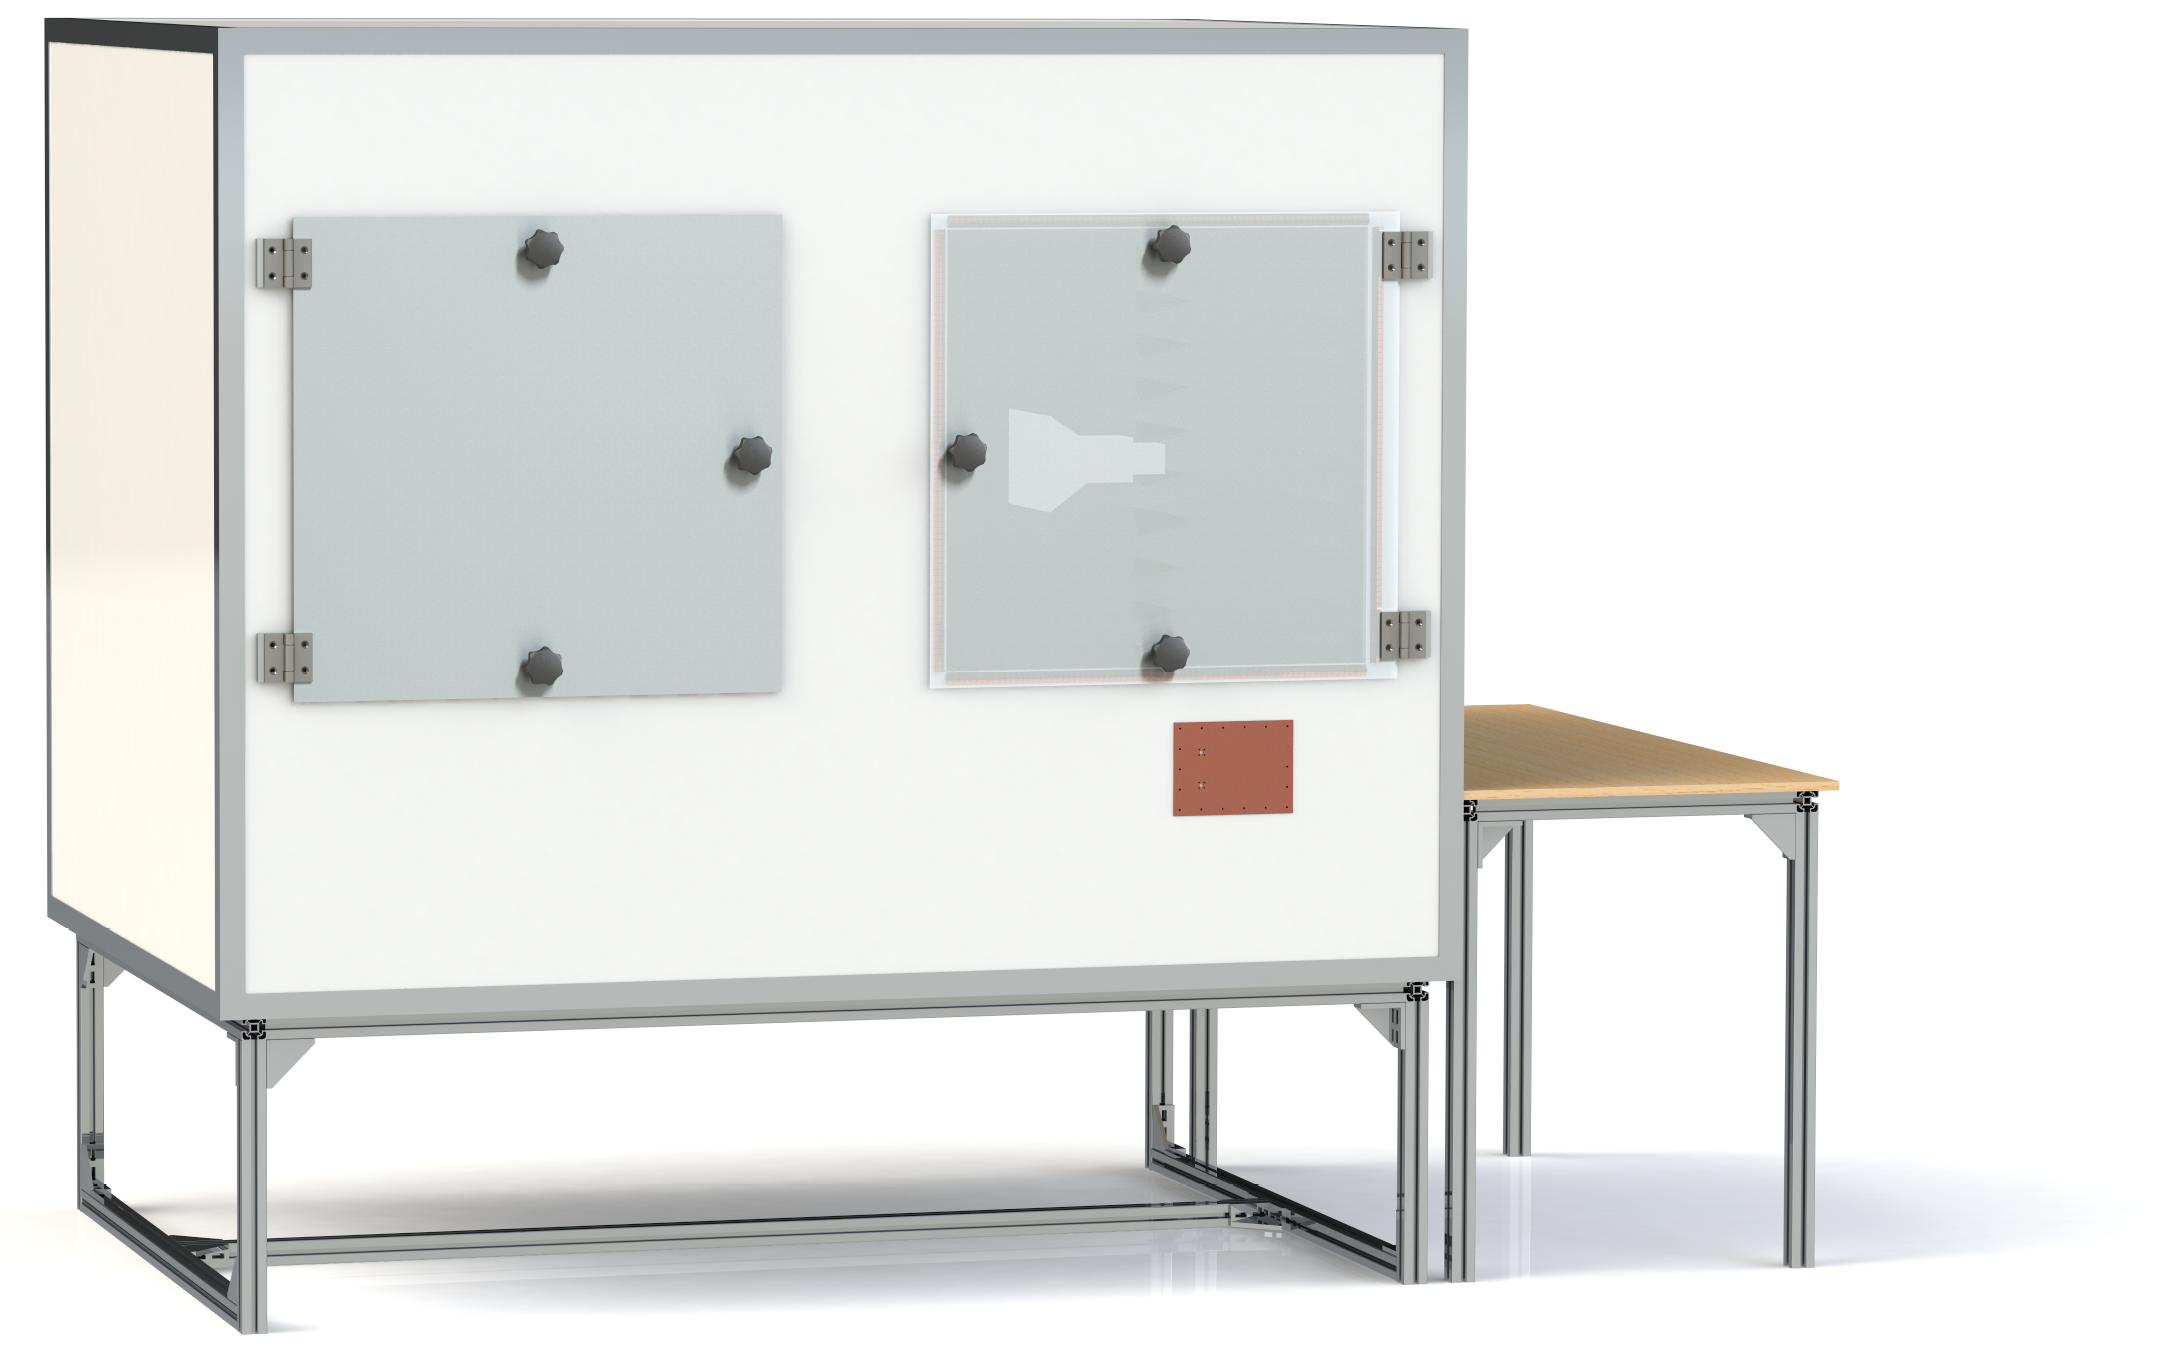
\includegraphics[width = .7\textwidth, trim = 0cm 0cm 1cm 0cm, clip]{Abbildungen/Kapitel3/Absorberkammer_Frontansicht.png}
    \caption{CAD-Modellansicht des Versuchsstandes}
    \label{fig:3_Entwurf_CAD}
\end{figure}



%Türen

%Dichtungen

%Kabeldurchführungen

%Gestell

%Beleuchtung












\section{Ausarbeitung}\label{cha:3_Ausarbeitung}


Die Detaillierung des Entwurfes basiert größtenteils auf den Spezifikationen und Maßen verfügbarer Kaufteile und den Abschätzungen für gewählte Abmessungen anhand von Ausführungen oder Beispielen in den herangezogenen Veröffentlichungen. Dabei sind vor allem~\cite{Design_of_shielded_enclosures, EMV-gerechtes_Geraetedesign, EM_Schirmung, Simplified_shielding, Handbook_Shielding_Materials_and_Performance} zu nennen, die als Referenz dienten. Im Folgenden wird das Ergebnis des Konstruktionsprozesses in einer möglichst systematischen Reihenfolge geschildert.

\subsection{Verwendete Messtechnik}

Die Hauptkomponente der verwendeten Messtechnik stellt, wie bereits erwähnt, ein \ac{VNA} dar. Der für diese Arbeit zur Verfügung stehende \ac{VNA} der Firma Anritsu ist ein Zweikanal-Netzwerkanalysator mit einem Arbeitsbereich zwischen \SI{1}{\mega\hertz} und \SI{20}{\giga\hertz}. Ein Auszug mit den für dieses Modell relevanten Daten und Diagrammen nach~\cite{VNA-Datenblatt} ist im \Anhang\ref{A:Datenblatt_VNA} zu finden. 
\par
\vspace{\linespace}
Da der \ac{VNA} mithilfe der zwei verfügbaren Ports sowohl die Sendeantenne speist als auch das Messsignal an der Empfangsanatenne aufnimmt, können die Streuparameter der Übertragung direkt ermittelt werden~(vgl. \Abschnitt\ref{cha:4_Allgemeines}). Außerdem wären Zeitbereichsmessungen (Time Domain Measurements) möglich, wodurch eine Unterscheidung zwischen direkten und indirekten Koppelpfad möglich ist~\cite{Techniques_Shielding_Effectiveness_Far_Field_Simulation}. %Im \Kapitel\ref{cha:4} wird darauf näher eingegangen.
\par
\vspace{\linespace}
% Die Kalibration der Messtechnik erfolgt mithilfe des zugehörigen Kalibrationskits, wodurch bei korrekter Durchführung die im Auszug des Datenblattes (vgl. \Anhang\ref{A:Datenblatt_VNA}) dargestellten Unsicherheiten eingehalten werden sollten. Auf die durchgeführte Kalibration des \ac{VNA} wird im \Abschnitt\ref{cha:4_Kalibration_Messtechnik} näher eingegangen.
% \par
% \vspace{\linespace}
Die Verbindung des \ac{VNA} erfolgt mittels der zugehörigen Signalkabel, die eine Wellenimpedanz von \SI{50}{\ohm} aufweisen~\cite{Testkabel_VNA-Datenblatt}. Die Anschlüsse sind \ac{SMA} kompatible Steckverbinder mit \SI{2,92}{\milli\meter}-Stecker.
\par
\vspace{\linespace}
%Antennen/Waveguides
    %Größe
    %Platziert mit vorhandenen Stativen
Die zur Verfügung stehenden Antennen sind Breitband-Hornstrahler mit einer linearen Polarisation und den in der \Tabelle\ref{tab:3_Spezifikationen_Antennen} zusammengefassten wichtigsten Spezifikationen nach~\cite{Antennen-Datenblatt}. Weitere Kenndaten sind im \Anhang\ref{A:Datenblatt_Antennen} zu finden. Die Antennen bieten ebenfalls einen SMA-Anschluss für die Signalkabel, welche nach~\cite{DIN_EN_61000-5-7} so ausgeführt sind, dass ihre Kopplungsdämpfung mit garantierten \SI{95}{\Dezibel}~\cite{Pasternack_Koaxkabel_PE-P142LL} deutlich über der zu messenden Schirmdämpfung liegt, wie an den Messwerten der Referenzmessungen in~\cite{FSS_Toedter_Diplomarbeit} erkennbar ist.  

\begin{table}[ht]
    \centering
    \caption[Technische Spezifikationen der verwendeten Hornstrahler]{Technische Spezifikationen der verwendeten Hornstrahler nach~\cite{Antennen-Datenblatt}}
    \label{tab:3_Spezifikationen_Antennen}
    \vspace{\tablespace}
    \begin{tabular}{p{6cm} p{4cm}}
    \toprule
        \textbf{Spezifikation} & \textbf{Wert} \\
    \midrule
        Frequenzbereich & $0,8 - 18\,\si{\giga\hertz}$ \\
        Halbwerts-Strahlbreite  & $111-13\si{\degree}$ (E-Feld) \\
                                & $78-10\si{\degree}$ (H-Feld) \\
        Kreuzpolarisation-Isolation & \SI{25}{\Dezibel} (typ.) \\
        Stehwellenverhältnis (VSWR) & $1,5 : 1$ (typ.) \\
        Abmessungen             & $244\times160,5\times228\,\si{\milli\meter}$ \\
    \bottomrule
    \end{tabular}
\end{table}

Mit den vorhandenen Aluminium-Stativen können die Antennen frei auf einer Höhe zwischen \SI{53}{\centi\meter} und \SI{158}{\centi\meter} platziert werden, was eine Positionierung in der Messkabine entsprechend der Anforderungen erlaubt.




\subsection{Konstruktion}\label{cha:3_sub_Konstruktion}

Die Modulwände werden hauptsächlich aus den Sandwichpaneelen gebildet, wodurch deren Auswahl von zentraler Bedeutung für die restliche Konstruktion ist. Aufgrund von Produktverfügbarkeiten mussten Verbundplatten aus Sperrholz mit metallischen Deckblechen, wie sie im Rahmen professioneller Absorberkammern zum Einsatz kommen, schon zu Beginn der Konzeptphase verworfen werden. Als Alternative wurden Wabenkernplatten gewählt, welche ebenfalls durchgehende Deckbleche besitzen, aufgrund ihrer inneren Struktur ein deutlich günstigeres Verhältnis aus Biegesteifigkeit und Gewicht besitzen und auf ganz ähnliche Weise verarbeitet werden können~\cite{Alucore-Datenblatt}. Im Messbereich zwischen 1 -- \SI{18}{\giga\hertz} sind nach \Abschnitt\ref{cha:2_sub_Schirmung_ebener_Wellenfelder} die Absorptions- und Reflektionsdämpfung für die kombinierte Blechstärke von \SI{2}{\milli\meter} bereits so hoch, dass für die real erreichte Schirmung des Versuchsstandes gegenüber Störquellen von außen nur noch Öffnungen wie Türen oder Verbindungsstellen entscheidend sind.  
\par
\vspace{\linespace}
Für den vorgesehenen Einsatzzweck musste die Polyesterlackschicht an allen Wirkflächen, d.h. allen Verbindungsflächen der Modulwände untereinander und allen weiteren Anschlussflächen, mechanisch entfernt werden. Um trotz der sich stets an Luftatmosphäre bildenden Oxidschichten einen leitfähigen Kontakt an allen Wirkflächen herzustellen, wurden Funktionselemente nach Möglichkeit miteinander verschraubt. Dabei kann im Fall von Aluminium bereits bei Vorspannkräften in einer Größenordnung von \SI{1000}{\newton} davon ausgegangen werden, dass die harten Oxidschichten aufreißen und Metall-Metall-Kontakt entsteht~\cite{Projektarbeit}. Aus diesem Grund wurde unter anderem ebenfalls von der Verwendung von Nieten abgesehen, wobei ein weiterer Grund die theoretische Möglichkeit eines Umbaus oder einer Erweiterung bei Verwendung lösbarer Verbindungen war. Weiterhin nutzen Schraubenverbindungen im Fall der Modulwände die Wabenstruktur der Sandwichpaneele besser aus, was zu einer deutlich erhöhten Stabilität führt, als dies bei einer Vernietung der Fall wäre. An den Türen gewährleisten die gewählten HF-Dichtungen aufgrund der Relativbewegung bei jedem Schließvorgang eine mechanische Entfernung der Oxidschichten.
\par
\vspace{\linespace}
Die Grundlage für die Auslegung der L-Profile entsprechend des gewählten Wirkkonzeptes für die Modulwände bildete der aus der Schraubenberechnung bekannte Rötscher-Kegel. Die Schenkellänge der Profile, welche die Wabenkernplatten an den Eckstößen miteinander verbinden, wurden nach den verfügbaren Profilmaßen so gewählt, dass sich der Verspannungskegel innerhalb der verschraubten Teile vollständig ausbilden kann und somit die Vorspannkraft der Schrauben möglichst großflächig in die Wabenkernplatte eingeleitet wird. Die \Abb\ref{fig:3_Verspannungskegel_L-Profile} zeigt dies anhand einer schematischen Darstellung zusammen mit den gewählten Profilmaßen und dem sich ergebenden Ersatzquerschnitt des Schraubverbandes. 
\par
\vspace{\linespace}

\begin{figure}[ht]
    \centering
    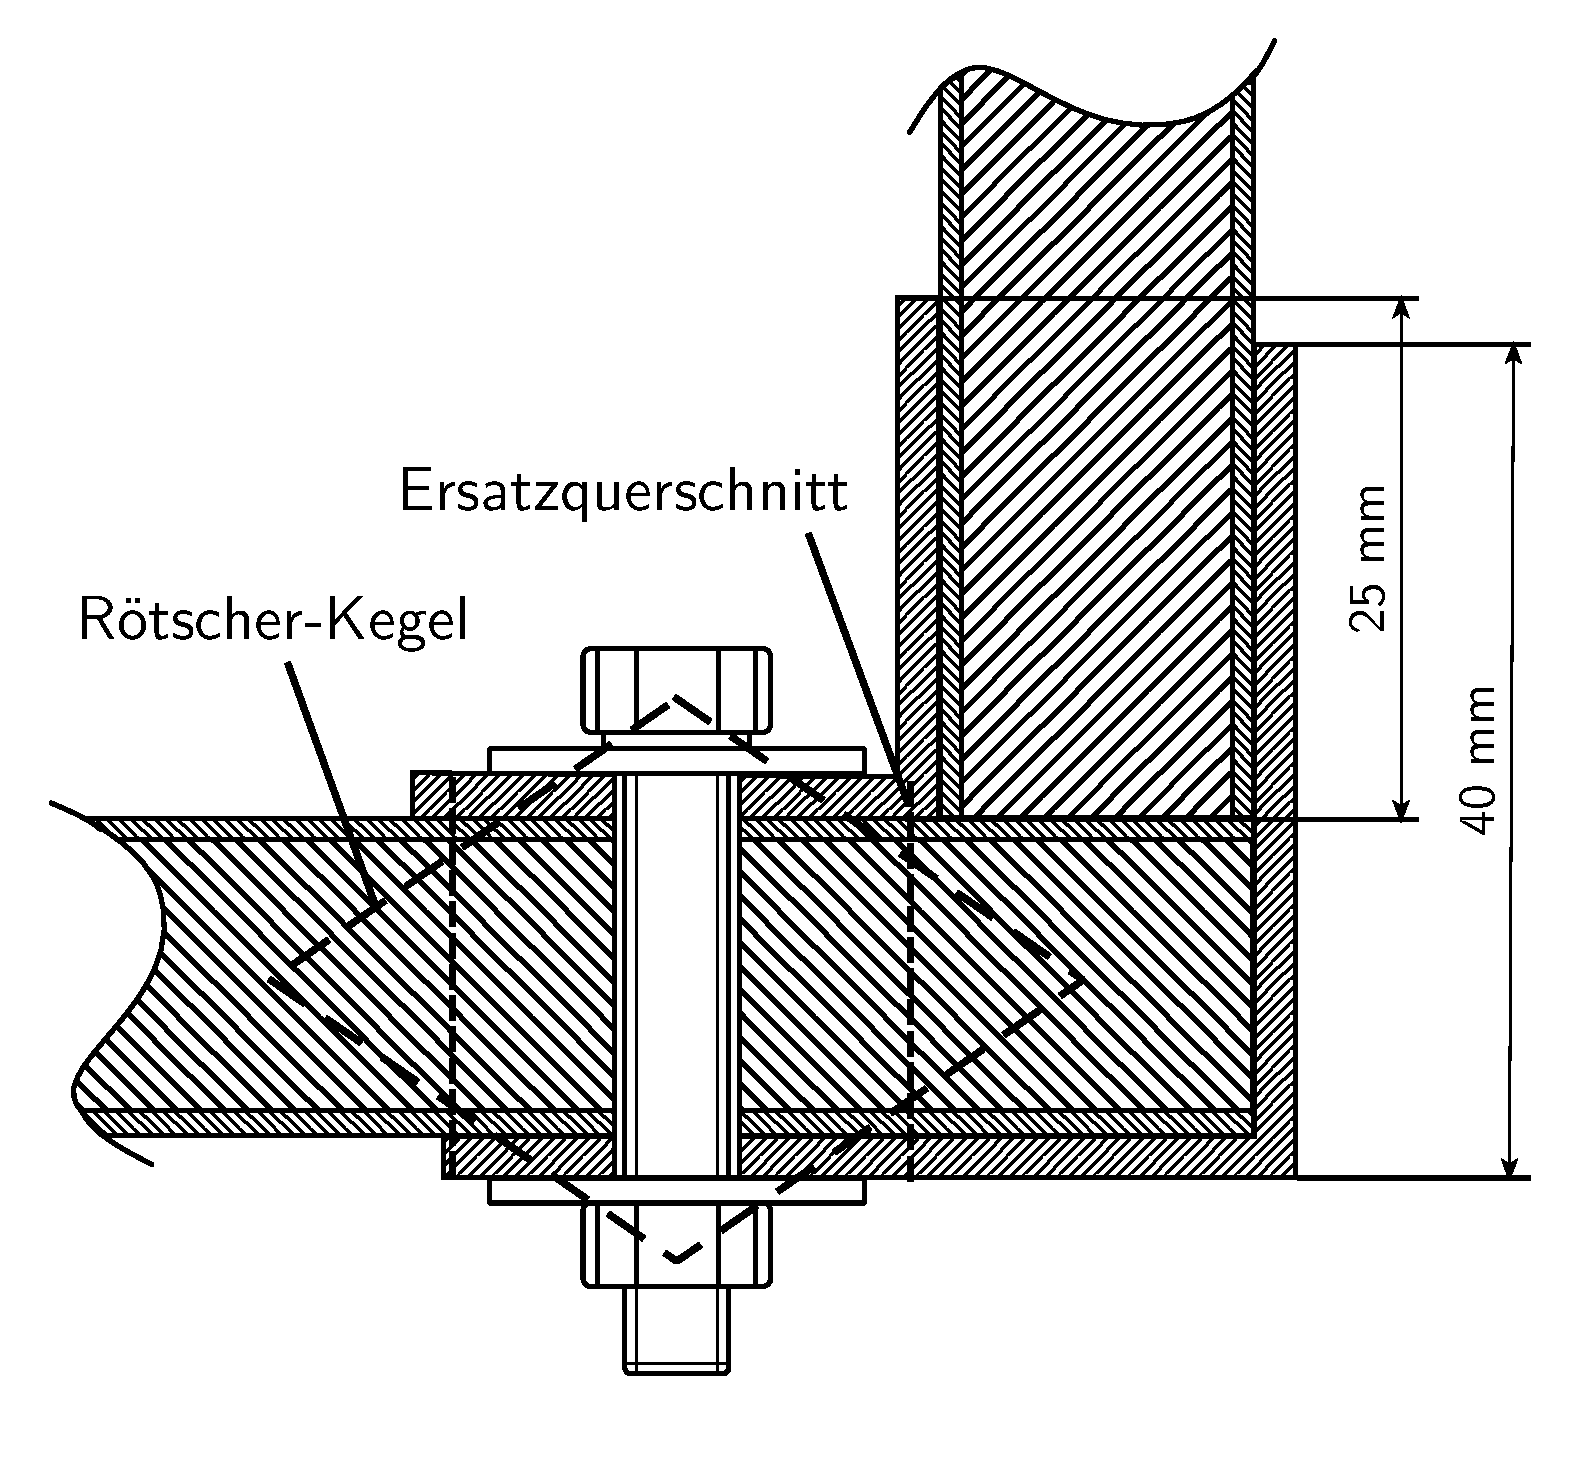
\includegraphics[page=1, trim=1cm 1.5cm 1cm 1cm, clip, width = .45\textwidth]{Abbildungen/Kapitel3/Schematik_Verspannungskegel.pdf}
    \caption{Schematische Darstellung des Verspannungsbereiches der verschraubten Modulwände}
    \label{fig:3_Verspannungskegel_L-Profile}
\end{figure}


Die Wahl des Schraubenabstandes wurde auf Grundlage eines Zusammenhanges nach~\cite{Design_of_shielded_enclosures} getroffen, welcher die erreichbare Schirmdämpfung als Funktion des Schraubenabstandes verschraubter Blechteile darstellt. Wie aus der Grafik in \Abb\ref{fig:3_Schirmwirkung_Schraubenabstand} hervorgeht, kann bei einem Schraubenabstand von \SI{10}{\centi\meter} von etwa \SI{70}{\Dezibel} theoretisch erreichbarer Schirmdämpfung je Funktionsfläche ausgegangen werden. Dieser Abstand wurde auch in Hinblick auf den Fertigungsaufwand der Bohrungen und Verschraubungen gewählt. Aufgrund der Sandwichbauweise der Modulwände befinden sich des Weiteren stets zwei versetzt verschraubte Wirkflächen im Koppelpfad, wodurch der Durchgriff weiter verringert wird. Die Anfertigung der Bohrungen erfolgte händisch und während des Zusammenbauprozesses, um eine möglichst exakte Ausrichtung der Bohrlöcher in den einzelnen verspannten Teilen relativ zueinander zu erreichen. Die Berechnung des Anzugsmomentes der Schrauben unter Beachtung der Druckfestigkeit der Wabenkernplatten stellte sicher, dass keine plastische Verformung des Wabenkerns erfolgte und die Wirkfläche somit eben blieb. Von der Verwendung selbstschneidender Schrauben wurde aufgrund der Gefahr verformter Gewinde und damit unsauberer Verbindungsstellen abgesehen.  
\par
\vspace{\linespace}\vspace{\linespace}

\begin{figure}[ht]
    \centering
    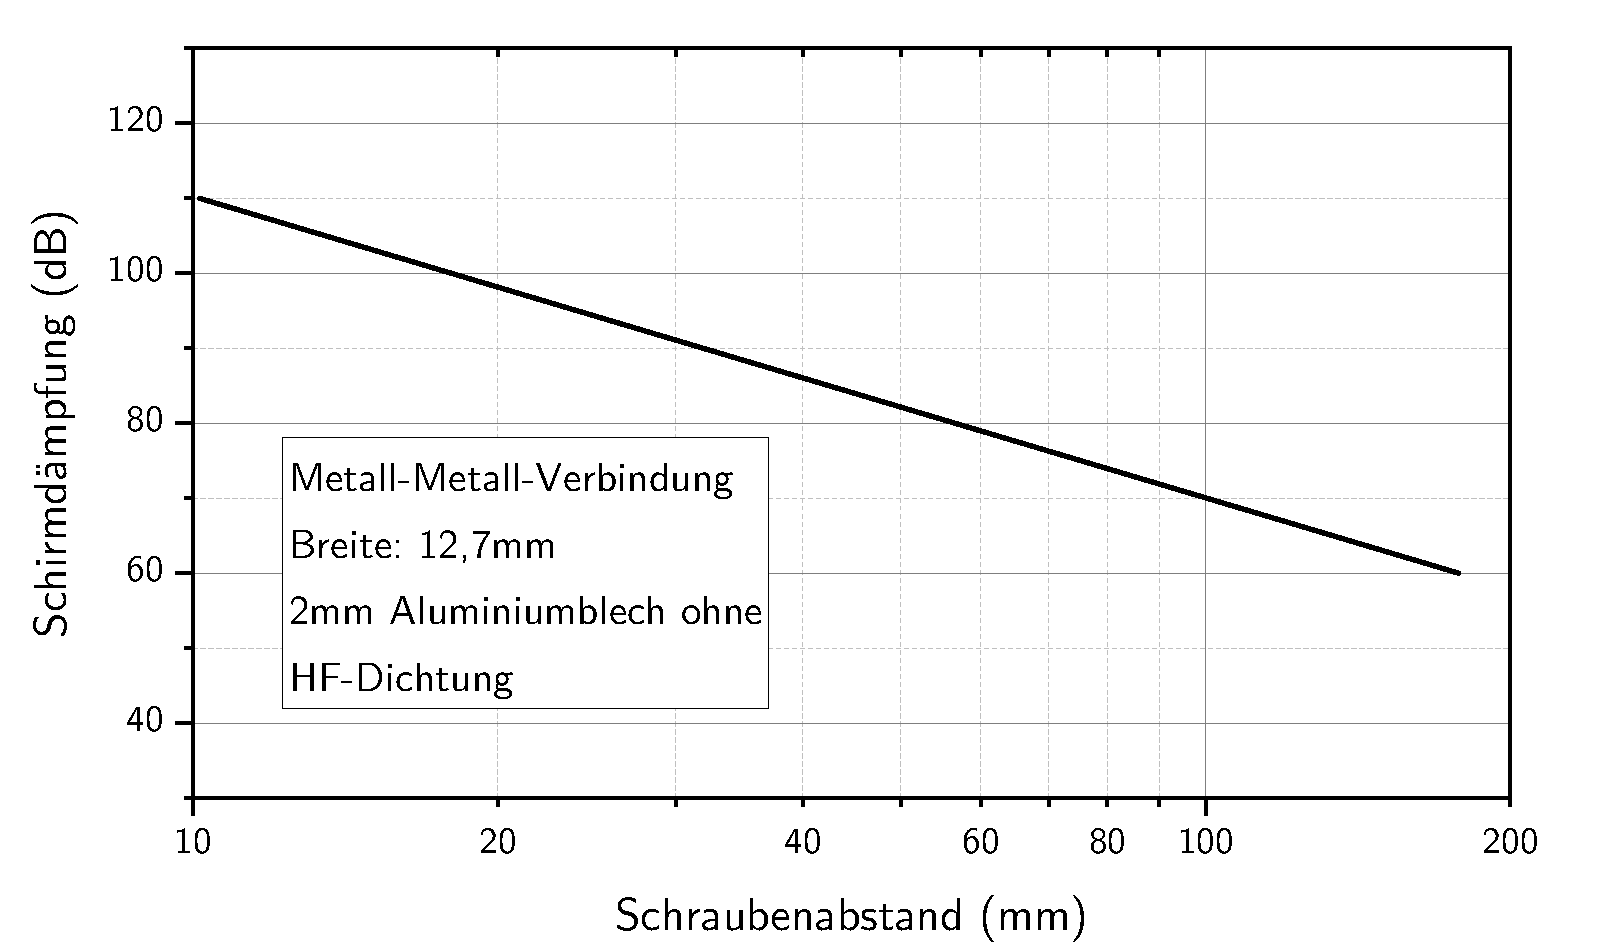
\includegraphics[page = 1, trim = 0cm 0cm 0cm 0cm, clip, width=.99\textwidth]{Abbildungen/Kapitel3/Schraubenabstand_Schirmwirkung.pdf}
    \caption[Schirmdämpfung verschraubter Blechteile in Abhängigkeit des Schraubenabstandes]{Schirmdämpfung verschraubter Blechteile in Abhängigkeit des Schraubenabstandes nach~\cite{Design_of_shielded_enclosures}}
    \label{fig:3_Schirmwirkung_Schraubenabstand}
\end{figure}


Um eine möglichst hohe Schirmdämpfung zu erreichen, wurde die Anordnung der Profile mit entsprechenden Aussparungen so gewählt, dass sich an keiner Stelle zwei Anschlussstellen im Koppelpfad von äußeren Störquellen nach innen direkt gegenüberstehen. Dies führt zu einer Labyrinthwirkung an Stellen von Profilübergängen und verringert somit ebenfalls den Felddurchgriff. Zusätzlich wurden auf der Innenseite alle Verbindungsstellen mit leitfähigem Aluminiumband versehen. Mit dem gewählten Konzept und Schraubenabstand wäre eine höhere Schirmwirkung an den Verbindungsstellen der Profile untereinander nur durch dichtes Verschweißen oder Verlöten zu erreichen~\cite{Design_of_shielded_enclosures, EM_Schirmung}, was jedoch schon zu Beginn der Konzeptphase aufgrund der Fertigbarkeit und unlösbaren Verbindung der Modulelemente als Fertigungsverfahren verworfen wurde. 
\par
\vspace{\linespace}


%Wabenkernplatten als Grundlage 
    %Verfügbarkeit
    %Vorteile gegenüber Vollmaterial (ggf. mit Grafik bzw. Wert
    %Datenblatt ggf. einfügen
    %Besonderheiten (Entfernen der Lackschicht z.B.)
    
%Aluprofile mit Rechnung bzw. der gewählten Dicke und Maßen

%Schraubenberechnung ggf.

%(Aufbau-(Reigenfolge))


Die Auswahl geeigneter Absorberelemente wurde unter Einbeziehung der erreichbaren Reflektionsdämpfung, der Höhe einzelner Elemente und ökonomischen Gesichtspunkten getroffen. Die Reflektionsdämpfung gibt hierbei das Verhältnis der Leistungen einer eintreffenden Welle und der reflektierten Teilwelle an. Eine möglichst hohe und gleichbleibende Reflektionsdämpfung über alle Einsatzfrequenzen ist dementsprechend wünschenswert. Im \Abschnitt\ref{cha:3_Entwurf} wurde die Auswahl bereits auf reine Pyramidenabsorber eingeschränkt. Zur Vermeidung von reflektivem Verhalten bei hohen Frequenzen sollten keine Absorberelemente mit abgeschnittener Spitze verwendet werden. 
\par
\vspace{\linespace}
Die gewählten Absorber besitzen die in \Tabelle\ref{tab:3_Reflektionsdaempfung_Absorberelemente} angegebene garantierte Reflektionsdämpfung im Messbereich dieser Arbeit. Mit einer Höhe von \SI{10}{\centi\meter}  verbleibt auch nach dem Einbau noch ein großer Messbereich in der Testkammer. Des Weiteren ist vor allem im höheren Frequenzbereich eine höhere Reflektionsdämpfung zu erwarten, als bei der \SI{20}{\centi\meter} hohen Variante der gleichen Produktfamilie. Auf die Verwendung noch höherer Elemente wurde aufgrund der steigenden Einschränkung des Messraumes und aus ökonomischer Sicht verzichtet.  
\par
\vspace{\linespace}

\begin{table}[ht]
    \centering
    \renewcommand{\arraystretch}{1.2}
    \caption[Gemessene und garantierte Reflektionsdämpfung der verwendeten EPP12 Pyramidenabsorber im Bereich zwischen \SI{1}{\giga\hertz} bis \SI{18}{\giga\hertz}]{Gemessene und garantierte Reflektionsdämpfung der verwendeten EPP12 Pyramidenabsorber im Bereich zwischen \SI{1}{\giga\hertz} bis \SI{18}{\giga\hertz} nach~\cite{Eco_Messtechnik_Absorber}}
    \label{tab:3_Reflektionsdaempfung_Absorberelemente}    
    \vspace{\tablespace}
    \begin{tabular}{p{2cm} C{1.6cm} C{1.6cm} C{1.6cm} C{1.6cm} C{1.6cm}}
        \toprule
            &   \multicolumn{5}{l}{\textbf{Reflektionsdämpfung [\SI{}{\Dezibel}]}} \\
        \midrule
            &   \SI{1}{\giga\hertz} & \SI{3}{\giga\hertz} & \SI{5}{\giga\hertz} & \SI{10}{\giga\hertz} & \SI{18}{\giga\hertz} \\
        \textbf{Gemessen}   &   15  &   32  &   42  &   50  &   55 \\    
        \textbf{Garantiert} &   12  &   30  &   40  &   45  &   50 \\
        \bottomrule
    \end{tabular}

\end{table}

Auf dem Messprotokoll~\cite{Eco_Messtechnik_Absorber} sind außerdem keine ausgezeichneten Peaks oder Einbrüche des Dämpfungsverhaltens zu erkennen. In Bezug auf Kosten und Abmessungen bieten vergleichbare, alternative Absorber ab etwa \SI{5}{\giga\hertz} nur eine um \SI{5}{\Dezibel} reduzierte Reflektionsdämpfung, was bei Betrachtung des Verhältnisses der Feldgrößen etwa einem Faktor 2 entspricht (vgl. \Tabelle\ref{tab:2_Relative_Pegel})~\cite{Holland_Shielding_Absorber}. Mit Ferritkacheln und zusätzlich darauf abgestimmten Hybridabsorbern kann zwar bereits im Frequenzbereich zwischen \SI{1}{\giga\hertz} bis \SI{3}{\giga\hertz} eine Reflektionsdämpfung von \SI{25}{\Dezibel} erreicht werden, jedoch ist mit dieser Kombination aufgrund der Impedanzabstimmung der PU-Absorber auf die Ferritkacheln bei höheren Frequenzen nur mit etwas mehr als \SI{30}{\Dezibel} zu rechnen, ab \SI{10}{\giga\hertz} sogar nur mit weniger als \SI{30}{\Dezibel}~\cite{Holland_Shielding_Absorber} und teils stark ausgeprägten Peaks in bestimmten Frequenzbändern. Aus diesen Gründen wurden die Absorber des Typs EPP12 der Firma \Firma{ECO-Messtechnik GmbH und Co. KG} verwendet. 
\par
\vspace{\linespace}
Für die Verkleidung von schmalen Bereichen und als Führung für die Antennenkabel, um eine stets gleichbleibende Lage über alle Messungen zu gewährleisten, kamen zusätzlich Flachabsorber des Typs EPF15, ebenfalls von \Firma{ECO-Messtechnik GmbH und Co. KG}~\cite{Eco_Messtechnik_Absorber}, zum Einsatz. Die Auskleidung der Ecken erfolgte mit versetzt angeordneten, umgedrehten Pyramidenstreifen. Dadurch konnte die nicht von Absorbern bedeckte Fläche auf ein Minimum reduziert und für die orthogonal angeordneten Elemente eine plane Anschlussfläche gewährleistet werden (vgl. \Abb\ref{fig:3_Absorberplatzierung}).
\par
\vspace{\linespace}

\begin{figure}[ht]
    \centering
    \includegraphics[draft = false, height=.2\textheight]{Abbildungen/Kapitel3/DSC_4536.jpg}
    \hspace{1cm}
    \includegraphics[draft = false, height=.2\textheight]{Abbildungen/Kapitel3/DSC_4523.jpg}
    \caption[Platzierung der verwendeten Absorber in Eckbereichen und an Durchführungen]{Platzierung der verwendeten Absorberelemente in Eckbereichen und an den Durchführungen}
    \label{fig:3_Absorberplatzierung}
\end{figure}


Die Befestigung der Absorberelemente erfolgte mittels Klettbändern, um eine nachträgliche Justierung oder einen Austausch leicht zu ermöglichen. Zusätzlich wurden Pyramidenabsorber im indirekten Koppelpfad der Antennen auf dem Boden platziert, um ungewollte Interferenz des direkten und indirekten Strahls zu verringern. Nach~\cite{Vergleich_Absorberhalle_Groundplane} erschien eine vollständige Auskleidung des Bodens auch in Hinblick auf Fertigung und Begehbarkeit in Ausnahmefällen nicht sinnvoll. Im dort durchgeführten Vergleich zeigt sich oberhalb von \SI{90}{\mega\hertz} ein qualitativ gleicher Verlauf der gemessenen Schirmdämpfung mit einem betragsmäßigen Unterschied von etwa \SI{5}{\Dezibel}. Durch Platzierung von wenigen Absorbern auf dem Boden zwischen den Antennen kann dies noch weiter reduziert werden. Der Unterschied zu einer Vollabsorberhalle ist dann kaum vorhanden. Darauf deuten auch die Ergebnisse in~\cite{Optimierung_Feldhomogenitaet} hin.
\par
\vspace{\linespace}




%Absorberelementauswahl 
    %Datenblatt
    %Anzahl Abschätzung
    %Flachabsorber für Ecken
    %Befestigung
    

Die am Reflektor zwischen den Antennen, welcher aus dem gleichen Material wie die Schirmwände besteht, befestigte Probenhalterung besteht aus zwei Z-Profile, in welche der nachfolgend beschriebene Probehalter eingeführt werden kann. Dies ermöglicht einen leichten Austausch und eine Messung in zwei Polarisationsrichtungen ohne die Proben zwischendurch neu verschrauben zu müssen. Weiterhin wird durch die verwendete Halterung die gleiche feste Anlage am Reflektor unabhängig der Stärke der Proben gewährleistet. Dies ist in Hinblick auf die Verwendbarkeit der Messkammer für Folien und Schäume von Bedeutung, da beide Arten von Proben sehr unterschiedliche Dicken aufweisen. Dies ist auch für die Gestaltung des Probenhalters ausschlaggebend.
\par
\vspace{\linespace}
Zur sicheren Positionierung der Proben in der Halterung wurde eine Verschraubung gewählt. Zwischen den verschraubten Hälften des Probenhalters sollten ebenfalls HF-Dichtungen angebracht werden. Um trotz unterschiedlicher Probenkörperstärke ein sicheres Anliegen der Kontaktfederstreifen zu gewährleisten, wurden die beiden Teile des Probenhalters als Blechwannen ausgeführt. Damit ist eine gewisse Relativverschiebung zwischen den Hälften je nach verwendeter Probe möglich, ohne die Anpresskraft auf die HF-Dichtungen zu verringern. Mit der verwendeten Probenhalterung können somit ohne Einschränkung Proben zwischen $0-14\,\si{\milli\meter}$ und $21-35\,\si{\milli\meter}$ mit einer Ausdehnung zwischen \SI{110}{\milli\meter}$\; \times \;$\SI{110}{\milli\meter} und \SI{130}{\milli\meter}$\; \times \;$\SI{130}{\milli\meter} vermessen werden, was den Anforderungen entsprechend der Anforderungsliste entspricht (vgl. \Abb\ref{fig:3_Probenhalterung_und_Reflektor}). 
\par
\vspace{\linespace}
Die Öffnung des Reflektors wurde unter Beachtung der Fresnel-Ellipse der Übertragung zwischen den Antennen~\cite{Taschenbuch_HF-Technik} etwas größer gewählt als die Öffnung des Probenhalters, um den direkten Koppelpfad nicht zusätzlich zu beinträchtigen (vgl. \Abb\ref{subfig:3_Probenhalter_Konfig1}). Die Fresnelzone der Funkübertragung ist ein Ellipsoid, in welchem Hindernisse die Ausbreitung elektromagnetischer Wellen aufgrund der Wellencharakteristik stören können, auch wenn direkte Sichtverbindung besteht. Im Bereich der ersten Fresnelzone wird der Großteil der Strahlungsenergie übertragen. Verdeckungen innerhalb dieser führen aufgrund von destruktiven Interferenzen zur Dämpfung des Signals an der Empfangsantenne, da direkte und indirekte, reflektierte Strahlen eine Phasendifferenz von bis zu einer halben Wellenlänge aufweisen~\cite{Advanced_Elecronic_Communication_Systems}. Aufgrund der Probengröße ist eine Interaktion des Probenhalters mit der Fresnelellipse erster Ordnung bei niedrigen Frequenzen nicht zu vermeiden, da diese selbst geringsten Abständen zur Empfangsantenne einen Radius deutlich größer als \SI{10}{\centi\meter} aufweist. Der Radius der n-ten Fresnelzone lässt sich dabei mithilfe der Antennenabstände $d_1$ und $d_2$ von der Probe abschätzen~\cite{Taschenbuch_HF-Technik}

\begin{equation}
    r^F_n = \sqrt{\frac{n\cdot \lambda\cdot d_1 \cdot d_2}{d_1 + d_2}}\; \text{.}
    \label{Fresnelzone}
\end{equation}

\par
\vspace{\linespace}
Der Reflektor wurde mittels eines Gestells aus Holz in der Kammer platziert, um die Beeinträchtigung der Feldhomogenität zu minimieren. Durch möglichst genaue Messungen wurden die Anforderungen hinsichtlich der Positionierung von Antennen und Reflektor sichergestellt. Die Mobilität des Reflektors erlaubt die Nutzung einer ungeteilten Absorberkammer für anderweitige Messungen.
\par
\vspace{\linespace}

\begin{figure}[ht]
    \centering
    \begin{subfigure}[b]{0.9\textwidth}
        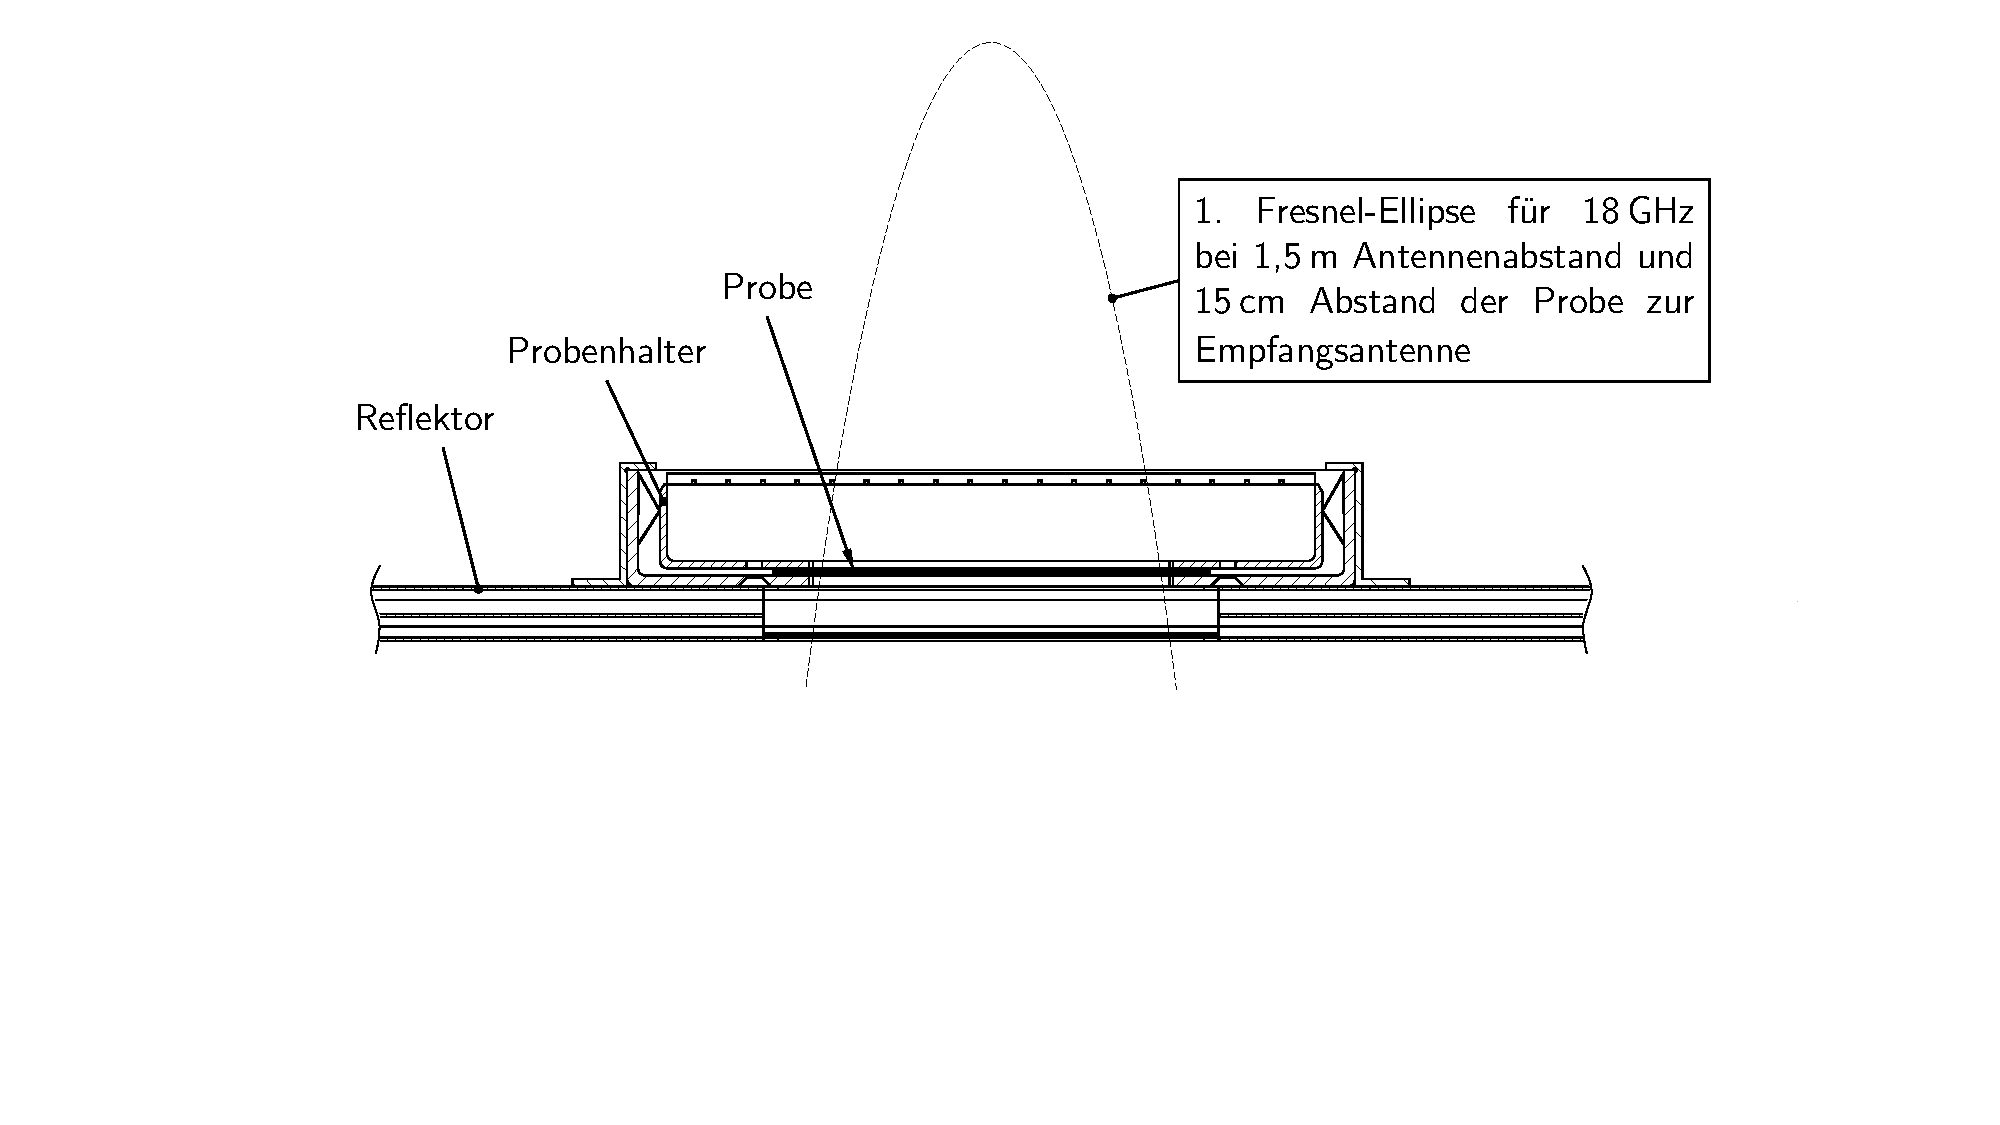
\includegraphics[page = 1, width=\textwidth, trim = 4.3cm 7cm 4.8cm 0cm, clip]{Abbildungen/Kapitel3/Probenhalter.pdf}
        \caption{Konfiguration 1 für Proben bis \SI{14}{\milli\meter} mit erster Fresnel-Ellipse}\label{subfig:3_Probenhalter_Konfig1}
    \end{subfigure}
    \hspace{2cm}
    \begin{subfigure}[b]{0.85\textwidth}
        \includegraphics[page = 2, width=\textwidth, trim = 5cm 7cm 5.5cm 7cm, clip]{Abbildungen/Kapitel3/Probenhalter.pdf}
        \caption{Konfiguration 2 für Proben bis \SI{35}{\milli\meter}}\label{subfig:3_Probenhalter_Konfig2}
    \end{subfigure}
    \caption{Schematische Darstellung der Probenhalterung in den möglichen Konfigurationen}
    \label{fig:3_Probenhalterung_und_Reflektor}
\end{figure}
    
%Probenreflektor mit Probenhalterung (CAD ggf.) und Beschreibung der Probenhalterung mit Vorteil der verschiedenen Dicken der Probekörper

%ggf. Prositionierung der Antennen (Stativ aus Holz)


Die Abmessungen der Durchführungen ergeben sich aus dem gewählten lichten Maß (vgl. \Abschnitt\ref{cha:3_Entwurf}) und den Maßen der verwendeten Kontaktfederstreifen. Um eine zu große Verformung der Kontaktfedern zu vermeiden, wurden Abstandshalter im Bereich der Scharniere so ausgelegt, dass die Türblätter bei korrekter Lage daran anliegen und sich nur unter erheblich größerem Kraftaufwand weiter als notwendig schließen lassen. Dies reduziert die Gefahr zu stark verformter HF-Dichtungen. Darüber hinaus wurden an allen drei verbliebenen Seiten Verschlüsse und damit Haltepunkte gegen den Liniendruck der Kontaktfedern vorgesehen, um die Verformung der Tür so weit wie möglich zu reduzieren und einen gleichmäßigen Anpressdruck an allen Seiten zu gewährleisten. Die Materialstärke wurde als Kompromiss aus Steifigkeit und Gewicht gewählt. Die herausgeschnittenen Stücken der Modulwand konnten nicht als Türblätter genutzt werden, da ihr Maß höchsten dem lichten Maß der Durchführung entspricht und somit keine Möglichkeit für das Einbringen von Dichtungen bestanden hätte.
\par
\vspace{\linespace}


%Türen mit Verschlüssen
    %Begründung Anzahl Verschlüsse
    %Detail mit Abstandshalter der Scharniere (damit Kontaktfederstreifen nicht zusammengedrückt werden)

Für die Schnittstellen der Antennenkabel an der Messkabine wird u.a. in~\cite{EM_Schirmung, EMV} die Verwendung einer Kupferplatte empfohlen, die aufgrund des sehr geringen Widerstandes Störströme gut ableiten kann. Dies bietet weiterhin den Vorteil, dass neue Schnittstellen direkt in der Kupferplatte hinzugefügt werden \mbox{können}, ohne dass die komplette Schirmwand nochmals bearbeitet werden muss. Die verwendete Platte wurde dementsprechend etwas größer als notwendig vorgesehen. Von Kabeldurchführungen an unterschiedlichen Stellen des Schirms wird in~\cite{EM_Schirmung, EMV, Design_of_shielded_enclosures} ausdrücklich abgeraten, sodass hier die Durchführung aller Anschlüsse an einem gemeinsamen Knoten erfolgt. Als Konnektoren wurden solche mit der gleichen Impedanz von \SI{50}{\ohm} wie die Anschlüsse des \ac{VNA} gewählt, um Rückreflektionen aufgrund von Impedanzsprüngen zu verringern. 
\par
\vspace{\linespace}
Zur Reduktion störender Einflüsse und reflektive Flächen wurde auf die Einführung eines Netzkabels und die feste Installation eines Halogenstrahlers zugunsten einer mobilen Beleuchtung verzichtet, falls diese für den Aufbau oder Modifikationen notwendig sein sollte. Für den Austausch der Proben gelangt ausreichend Licht durch die Türen in die Kammer. LED-Leisten könnten innerhalb der Kammer als Linienantennen und damit ebenfalls störend wirken. Ein ähnliches Vorgehen wird im Neuroimaging Center der Fakultät Psychologie und der Medizinischen Fakultät der TUD bei der Elektro\-enzephalo\-graphie angewandt. Weiterhin sind keine Lüftungen zusätzlich zu den Durchführungsöffnungen notwendig, da die Messkammer i.d.R. nicht betreten wird und in keinem Falls als Dauerarbeitsplatz genutzt wird~\cite{EM_Schirmung}. Die Regulierung von Temperatur und Luftfeuchtigkeit über die Schirmhülle und vorhandenen Öffnungen ist im Regelbetrieb ausreichend.  

%Auswahl Kabeldurchführungen (Impedanz von 50 Ohm im Match mit VNA --> Verweis Datenblatt VNA und Kabeldurchführungen (Muss matchen, um keine Rückreflektion zu bekommen (siehe Folien von Connector Care))
    %ggf. Detail mit Kupferplatte hierhin und nicht in Entwurf
    
\par
\vspace{\linespace}

Mithilfe der dargestellten konstruktiven und fertigungstechnischen Details konnten alle an das Design gestellten Anforderungen erfüllt werden. Weiterhin wurde darauf geachtet, Quellen für mögliche Messunsicherheiten und Feldinhomogenitäten so weit wie möglich zu verringern. Durch die Auswahl der Wirkkonzepte und Materialien konnte das Budget für den Versuchsstand eingehalten werden. Gegenüber einem Angebot von EMC Technik und Consulting GmbH für eine Absorberkammer gleicher Größe über ca. \SI{37000}{\text{\euro}} belaufen sich die Gesamtkosten für den fertigen Aufbau auf etwa ein Viertel. 
\par
\vspace{\linespace}
Die \Abb\ref{fig:3_Gesamtversuchsstand} zeigt Ansichten der äußeren Schirmhülle und der inneren Messstrecke als Haupt\-elemente des fertigen Versuchsstandes. Weitere Detailansichten, technische Zeichnungen der gefertigten Bauteile sowie ein Dokument mit Nutzungshinweisen befinden sich im digitalen Anhang auf der CD.
\par
\vspace{\linespace}

\begin{figure}[ht]
    \centering
    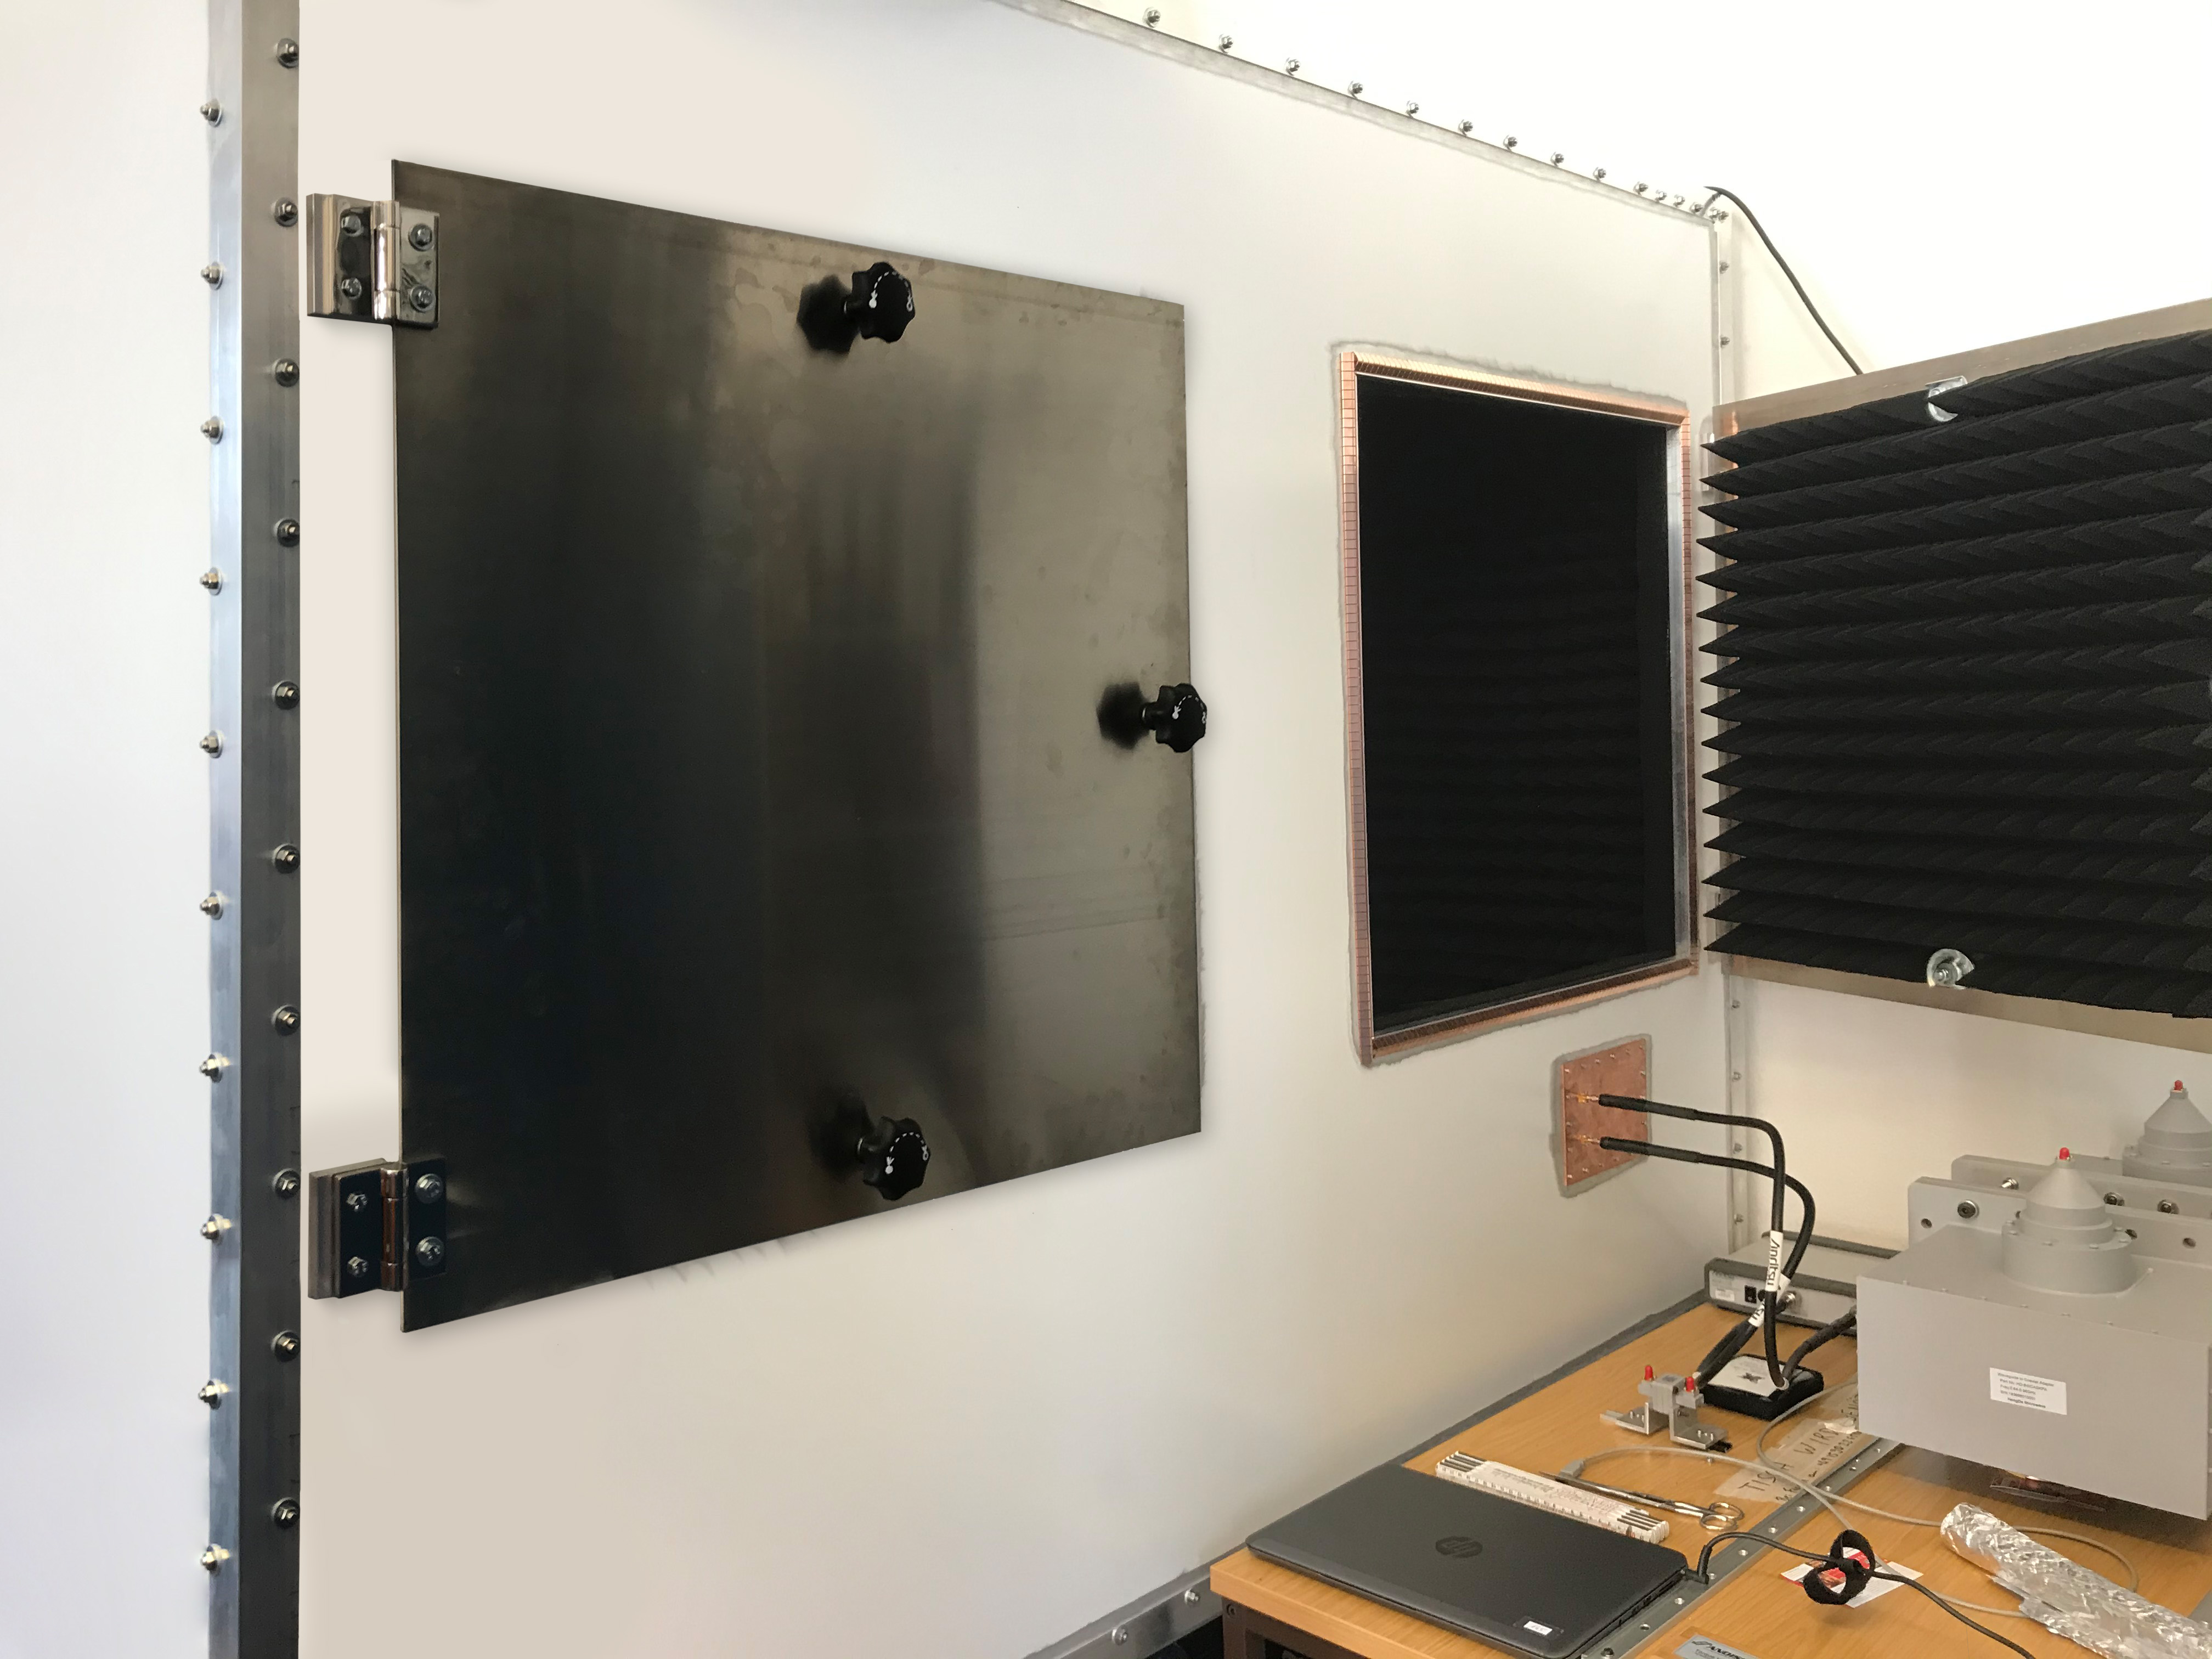
\includegraphics[height=.22\textheight, draft = false]{Abbildungen/Kapitel3/IMG_5467_bearbeitet.jpg}
    \hspace*{1cm}
    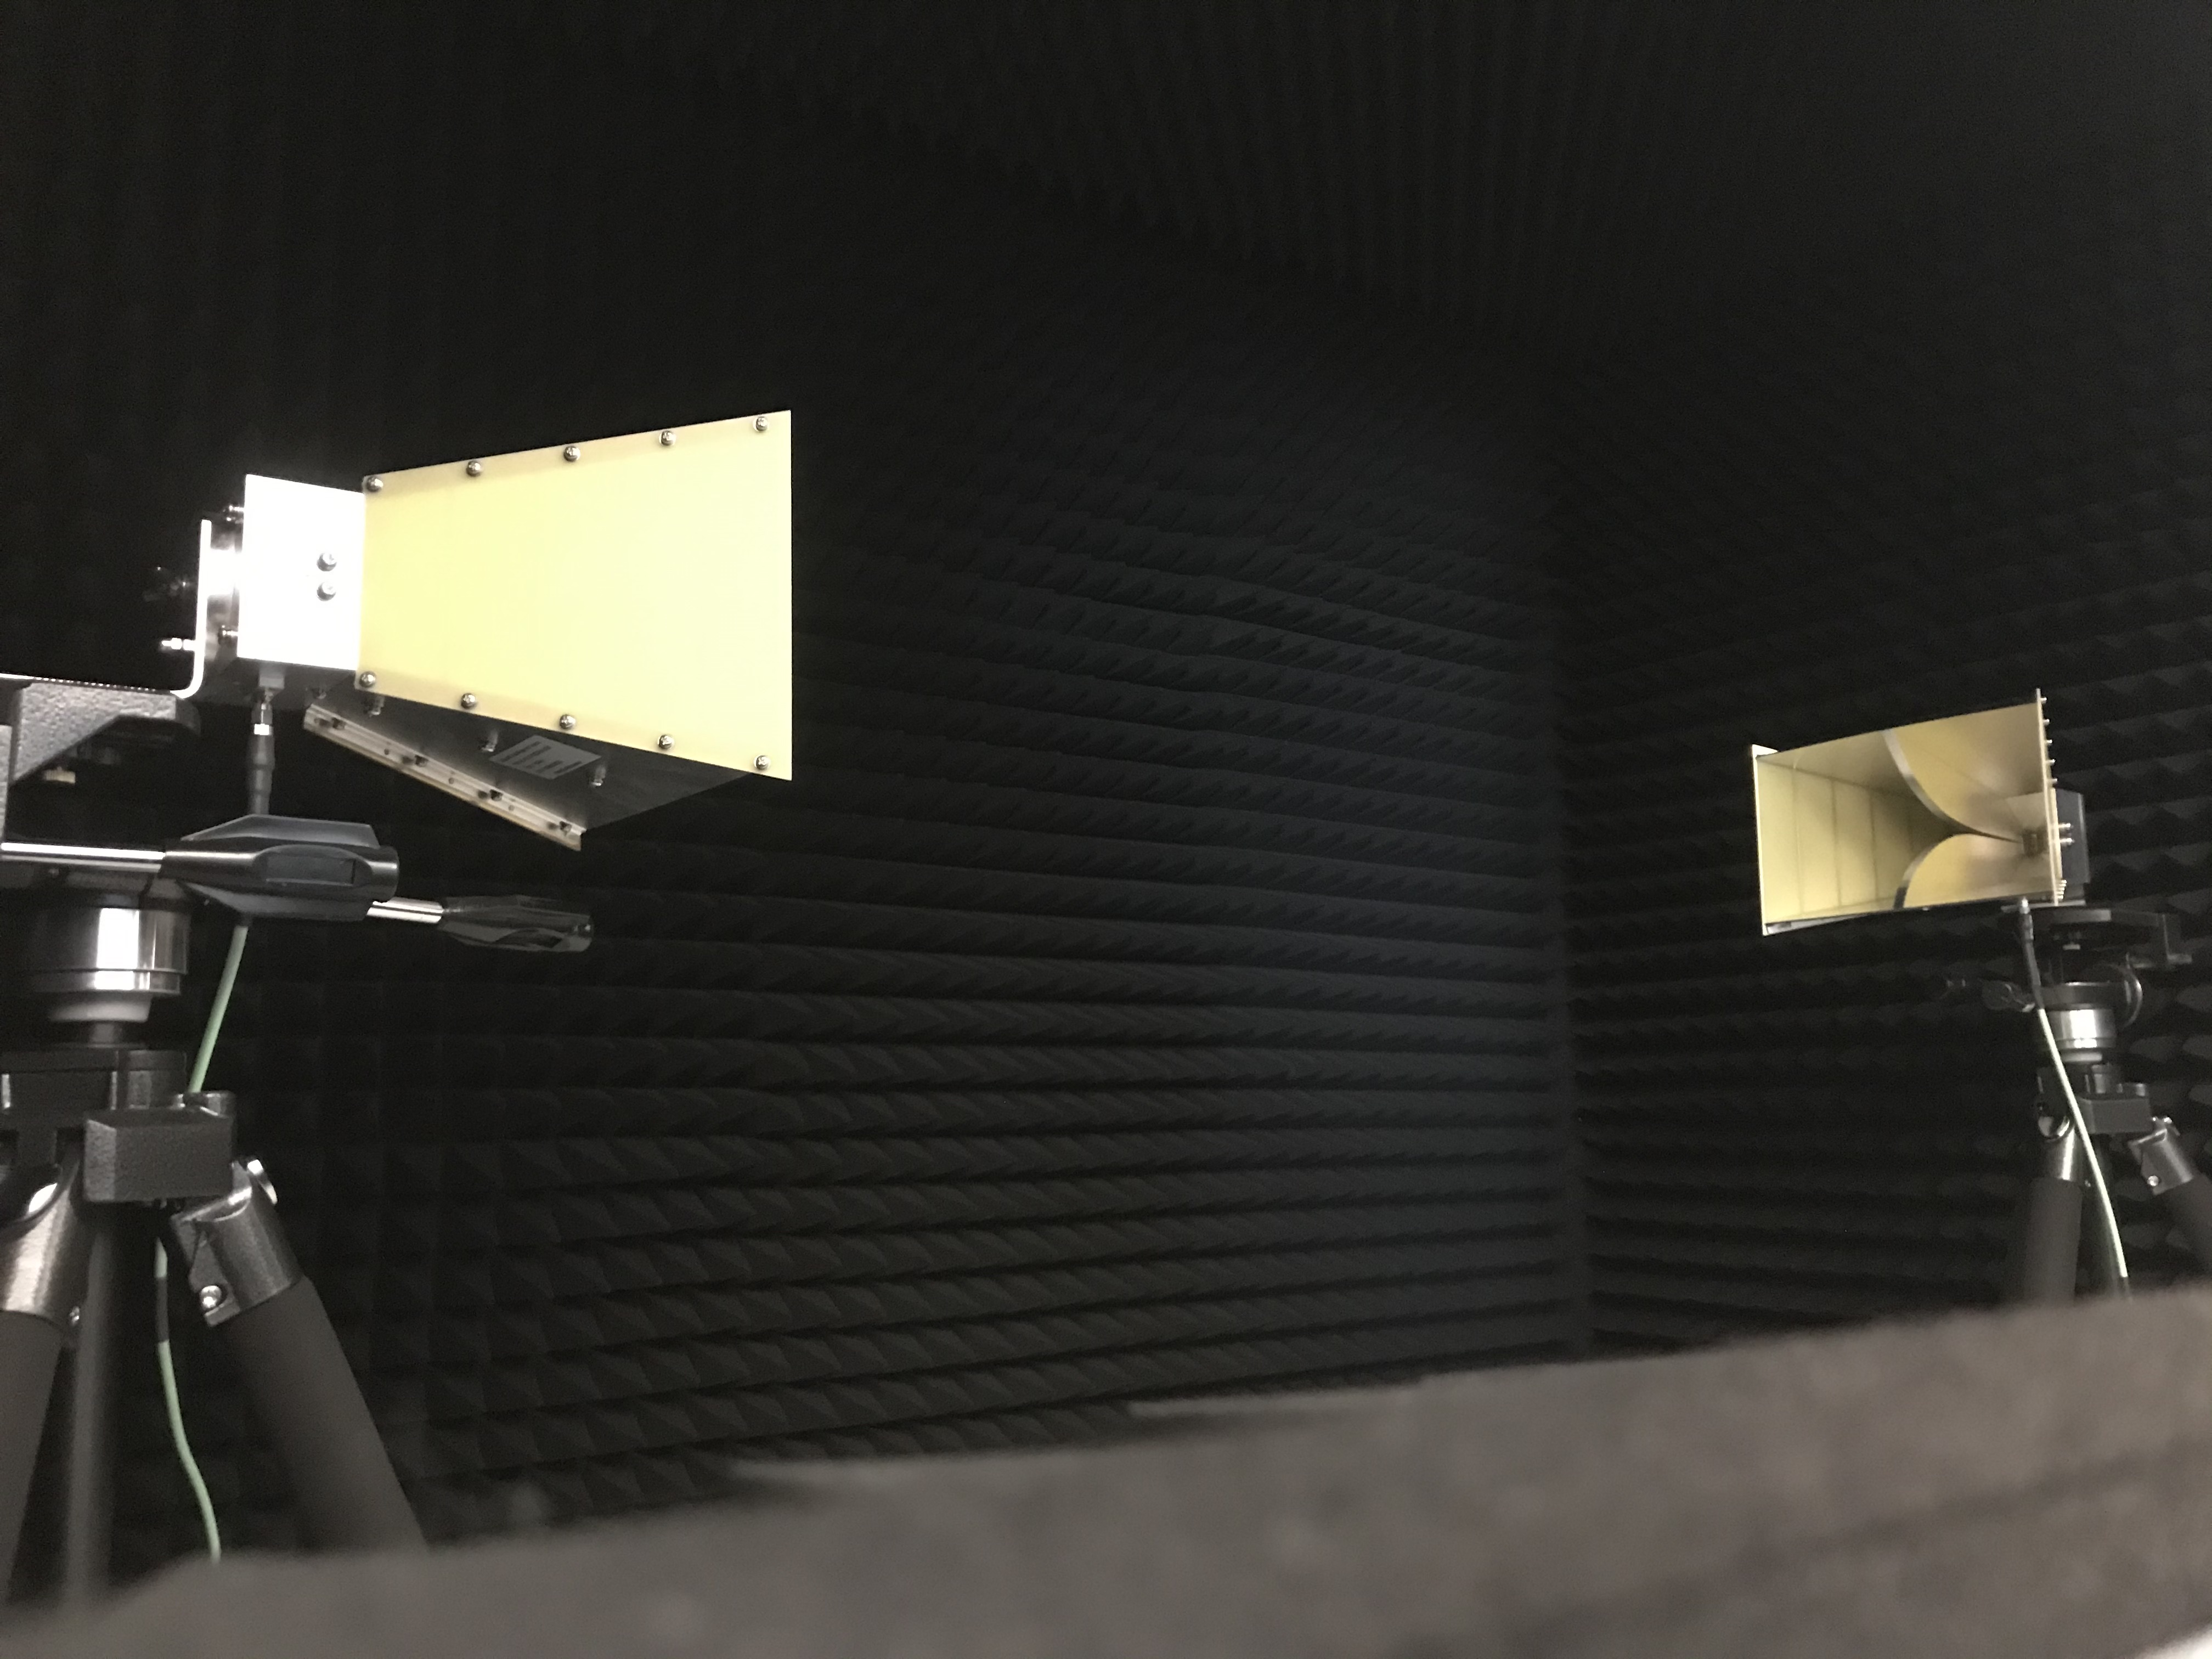
\includegraphics[height=.22\textheight, draft = false]{Abbildungen/Kapitel3/IMG_5472.jpg}
    \caption[Fernfeldversuchsstand von außen und Messstrecke]{Fernfeldversuchsstand von außen und Messstrecke mit Antennen}
    \label{fig:3_Gesamtversuchsstand}
\end{figure}



